\documentclass[journal,a4paper]{IEEEtran}

\usepackage{import}
\usepackage{graphicx}
\usepackage{xcolor}
\usepackage{soul}
\usepackage{times}
\usepackage{epsfig}
\usepackage{amsfonts}
\usepackage{amssymb}
\usepackage{colortbl}
\usepackage{upgreek}
\usepackage{booktabs}
\usepackage{multicol}
\usepackage{lipsum}
\usepackage{cite}
\usepackage{amsmath}
\usepackage[cmintegrals]{newtxmath}
\usepackage{bm}
\usepackage{url}
\usepackage{subfig}
\usepackage{multirow}
\usepackage{array}
\usepackage{pifont}
% it is comment.
% this is my comment.

\ifCLASSINFOpdf
  % \usepackage[pdftex]{graphicx}
  % declare the path(s) where your graphic files are
  % \graphicspath{{../pdf/}{../jpeg/}}
  % and their extensions so you won't have to specify these with
  % every instance of \includegraphics
  % \DeclareGraphicsExtensions{.pdf,.jpeg,.png}
\else
  % or other class option (dvipsone, dvipdf, if not using dvips). graphicx
  % will default to the driver specified in the system graphics.cfg if no
  % driver is specified.
  % \usepackage[dvips]{graphicx}
  % declare the path(s) where your graphic files are
  % \graphicspath{{../eps/}}
  % and their extensions so you won't have to specify these with
  % every instance of \includegraphics
  % \DeclareGraphicsExtensions{.eps}
\fi
\interdisplaylinepenalty=2500
% correct bad hyphenation here
\hyphenation{op-tical net-works semi-conduc-tor}
\DeclareRobustCommand*{\IEEEauthorrefmark}[1]{\raisebox{0pt}[0pt][0pt]{\textsuperscript{\footnotesize #1}}}

\begin{document}

%\title{Load Demand Estimation of LCC-Series Compensated WPT Systems using Front-End Measurements}
%\title{Transferred Power Estimation from an LCC Compensated Wireless Power Transmitter using Synchronized Sampling of the LCC Front-End Variables}
%\title{Estimation of the Transferred Power in LCC Compensated Wireless Power Transmitters using PWM-Synchronized Sampling of the LCC Variables}
\title{Estimation of the Transferred Power in LCC Compensated Wireless Power Transmitters with the use of PWM-Synchronized Sampling Technique}

% 	\author{\IEEEauthorblockN{
%         Farzad Farajizadeh,~\IEEEmembership{Student Member,~IEEE,}
%         D. Mahinda Vilathgamuwa,~\IEEEmembership{Fellow,~IEEE,}
%         Prasad Jayathurathnage,~\IEEEmembership{Member,~IEEE,}
%         and Gerard Ledwich, \IEEEmembership{Fellow,~IEEE}}
        
% 		\thanks{
% 			F. Farajizadeh, D. M. Vilathgamuwa, and G. Ledwich are with the Department of Electrical Engineering and Computer Science, Queensland University of Technology, Brisbane, QLD 4001, Australia (e-mail: f.faradjizadeh@gmail.com; mahinda.vilathgamuwa@qut.edu.au; g.ledwich@qut.edu.au).
% 		}
% 		\thanks{
% 			P. Jayathurathnage is with the Department of Electronics and Nanoengineering, School of Electrical Engineering, Aalto University, Espoo 00076, Finland (e-mail: prasad.jayathurathnage@aalto.fi).
% 		}
% 	}

% The paper headers

%\markboth{Journal of \LaTeX\ Class Files,~Vol.~14, No.~8, August~2015}%
%{Shell \MakeLowercase{\textit{et al.}}: Bare Demo of IEEEtran.cls for IEEE Communications Society Journals}


\maketitle

% As a general rule, do not put math, special symbols or citations
% in the abstract or keywords.
\begin{abstract}
In this paper, a new technique of synchronized sampling to estimate the transferred power in wireless power transfer (WPT) systems is proposed. Defining demand factor as a criterion linking unknown receiver parameters to the transferred power, it can be estimated by measuring the front-end variables of the transmitter LCC compensating network. Moreover, with the use of this technique, one does not need to know how the mutual inductance or load varies. As the demand factor is directly linked to the transferred power, the estimation of the demand factor can be considered as an increasingly effective way to control the flow of power in wireless power transfer systems. To prove the validity of this approach, a WPT system equipped with an LCC network to compensate the transmitter, and a series capacitor to compensate the receiver, is experimentally built and tested, and the results show a close consistency between the measured demand factor and the transferred power.  
\end{abstract}

% Note that keywords are not normally used for peerreview papers.
\begin{IEEEkeywords}
LCC Compensator, Load Estimation, Power Estimation, Resonant Converters, Soft-Switching, Wireless Power Transfer Systems.
\end{IEEEkeywords}

\IEEEpeerreviewmaketitle



\section{Introduction}

\IEEEPARstart{W}{ireless Power Transfer} (WPT) systems have drawn attention for many years. Attractive features, such as safety of consumer, ease of use, absence of mechanical connectors, immunity to harsh environments (e.g. dirt, chemicals, snow), flexibility in the receiver position, and dynamic power transmission, make industries and academia increasingly explore a vast number of remarkable ideas \cite{ADV_1,ADV_2,ADV_3,ADV_4}. In general, WPT research can be categorized into magnetic design of the WPT pads, transmitter and receiver compensation techniques, power electronic converters, and feedback and control techniques. %Some examples in each field are briefly reviewed as follows.

%To form an effective unidirectional WPT pad, Covic \textit{et al.} \cite{ADV_4} have proposed a novel magnetic design for polarized pads. Aiming to increase the transmitter-receiver distance, Kurs \textit{et al.} \cite{REPEATER} have proposed domino resonators. Taking the advantage of closely spaced transmitters, Farajizadeh \textit{et al.} \cite{Farzad} have proposed an approach to improved the transferred power profile. In the same work, a new type of N-Legged power electronic converter has been used and compensated to transfer power at a desirable level of soft-switching. For this purpose, the transmitter compensators are tuned with the use of ZCS compensating technique proposed by Pantic \textit{et al.} \cite{Pantic}. The compensators can also be used to make transmitters and receiver behave in a specific way, such as a current driven transmitter \cite{WPT_CDCD_Hou}, or voltage driven transmitter \cite{WPT_VD_LEE}, or coupling independent receiver \cite{LOAD_INDEPENDENT}.

\begin{figure}[t]
    \centering
    \subfloat[]{
        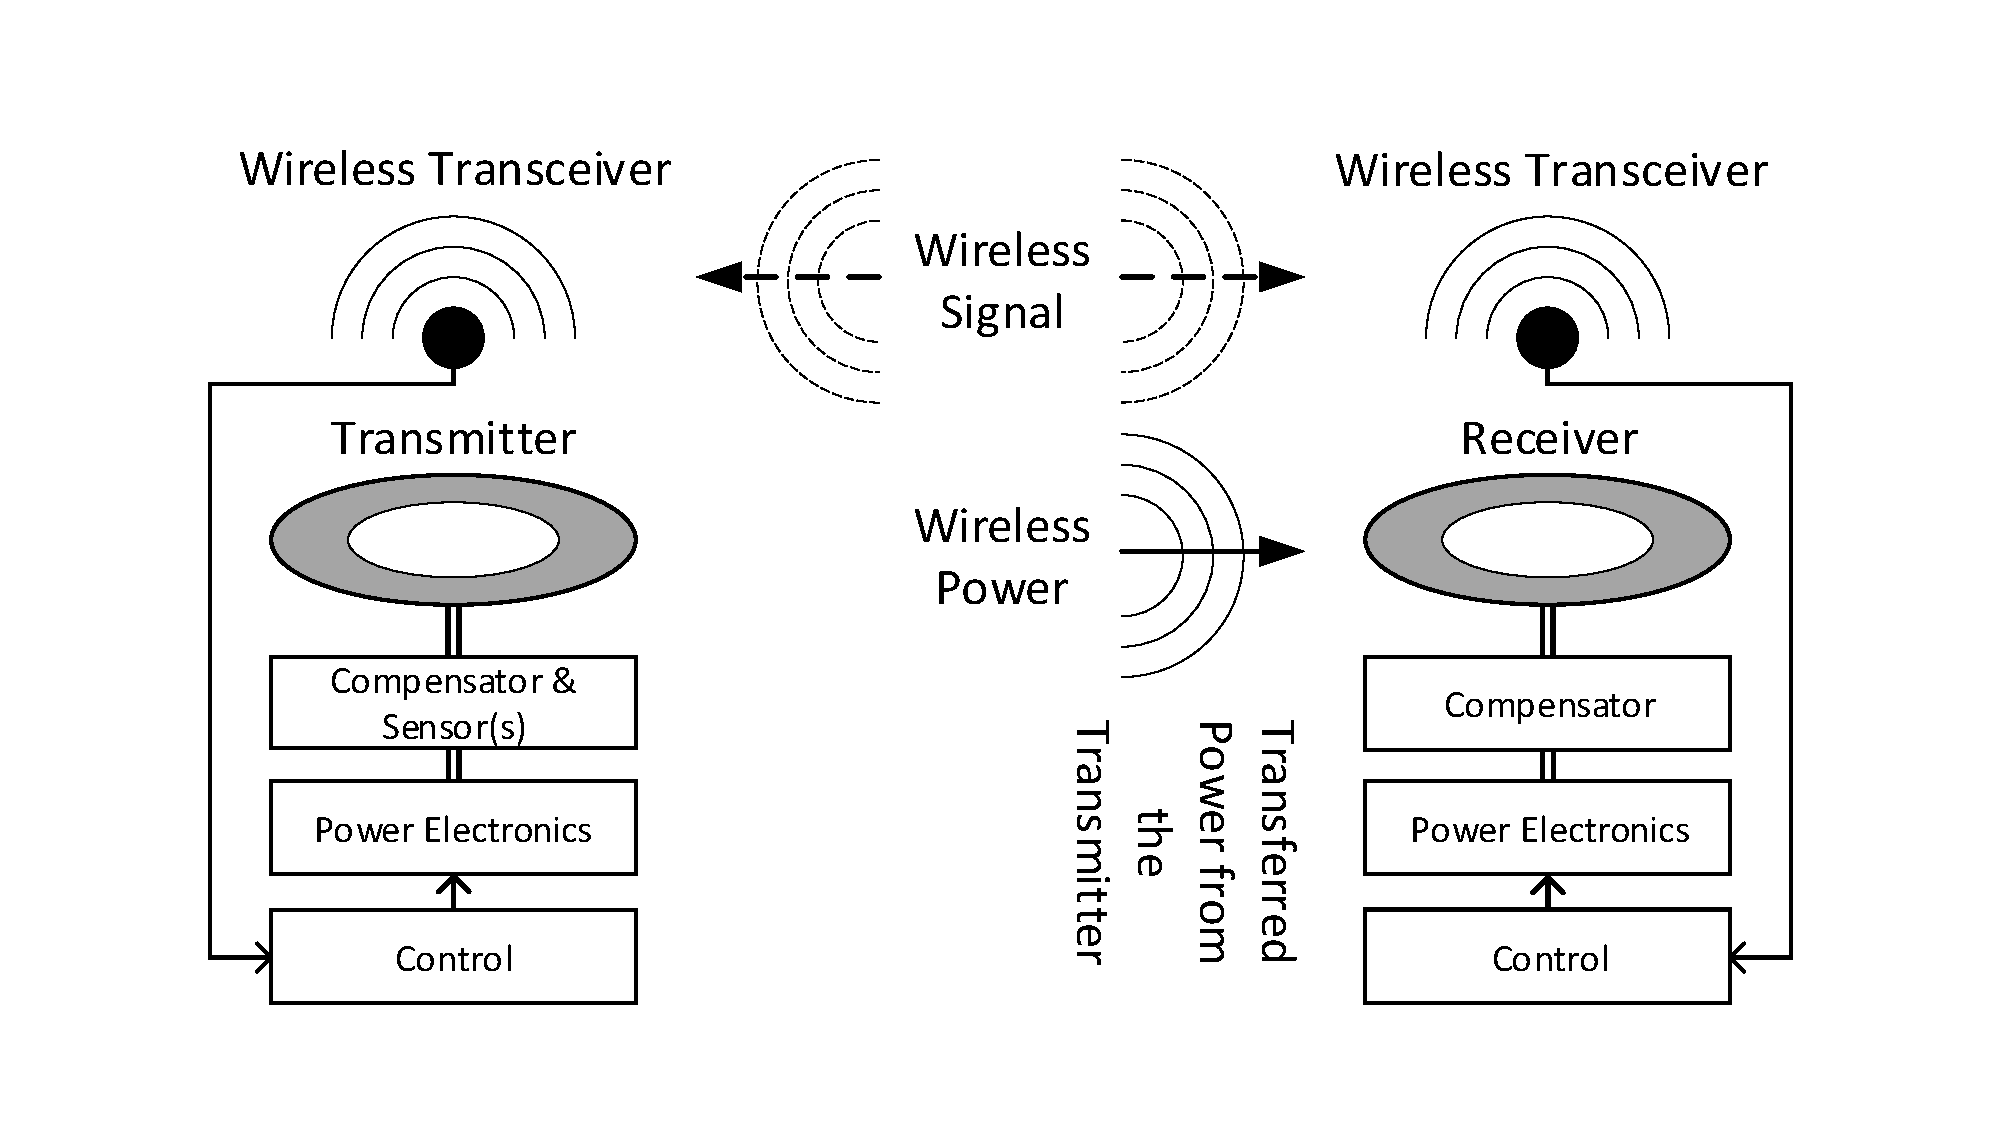
\includegraphics[clip, trim=1cm 1cm 1cm 1cm, width=1\columnwidth]{Figs/Fig1_a.pdf}
   %     \vspace{-6mm}
    }\\\vspace{-3mm}
    \subfloat[]{
%        \vspace{-6mm}
        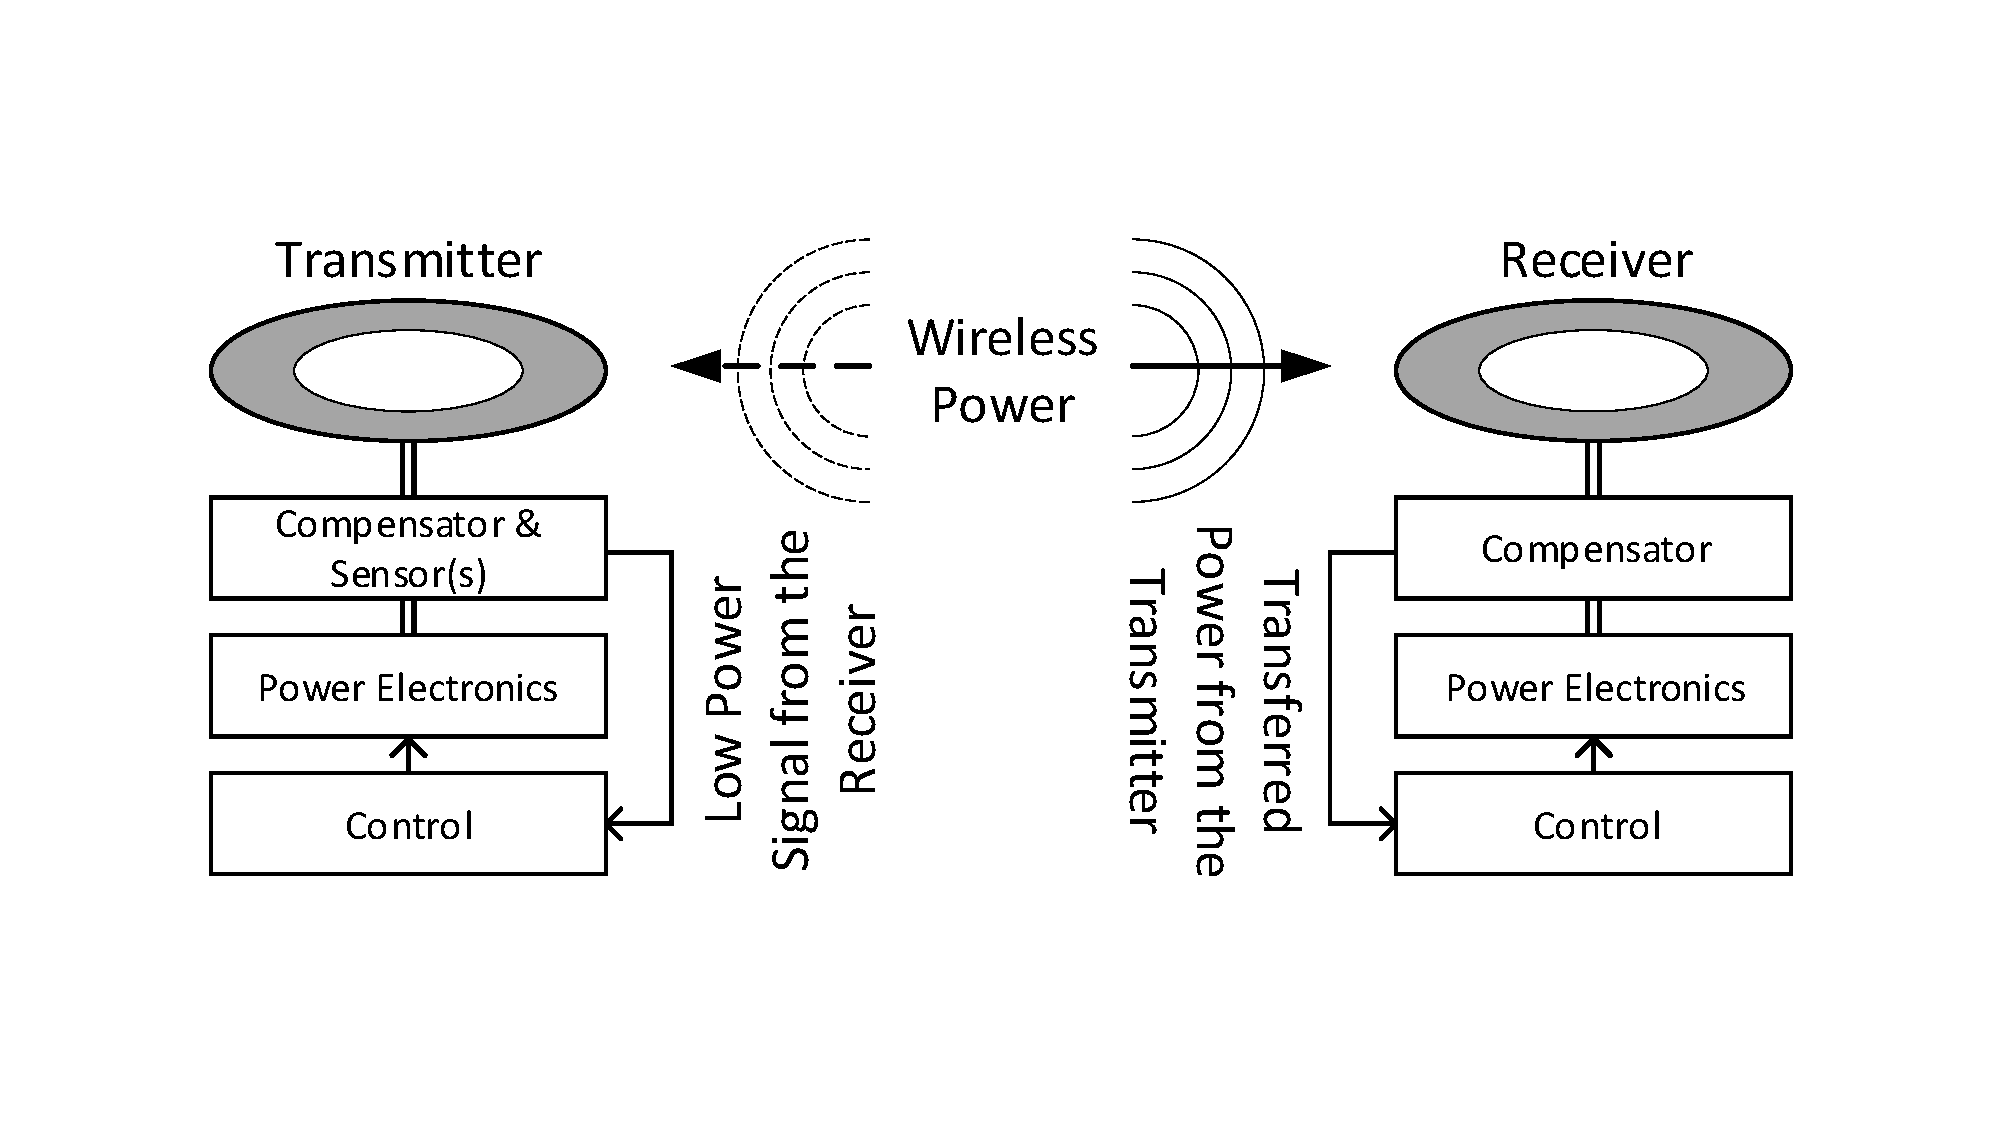
\includegraphics[clip, trim=0cm 3cm 0cm 3cm, width=1\columnwidth]{Figs/Fig1_b.pdf}
%        \vspace{-6mm}
    }\\\vspace{-3mm}
    \subfloat[]{
%        \vspace{-6mm}
        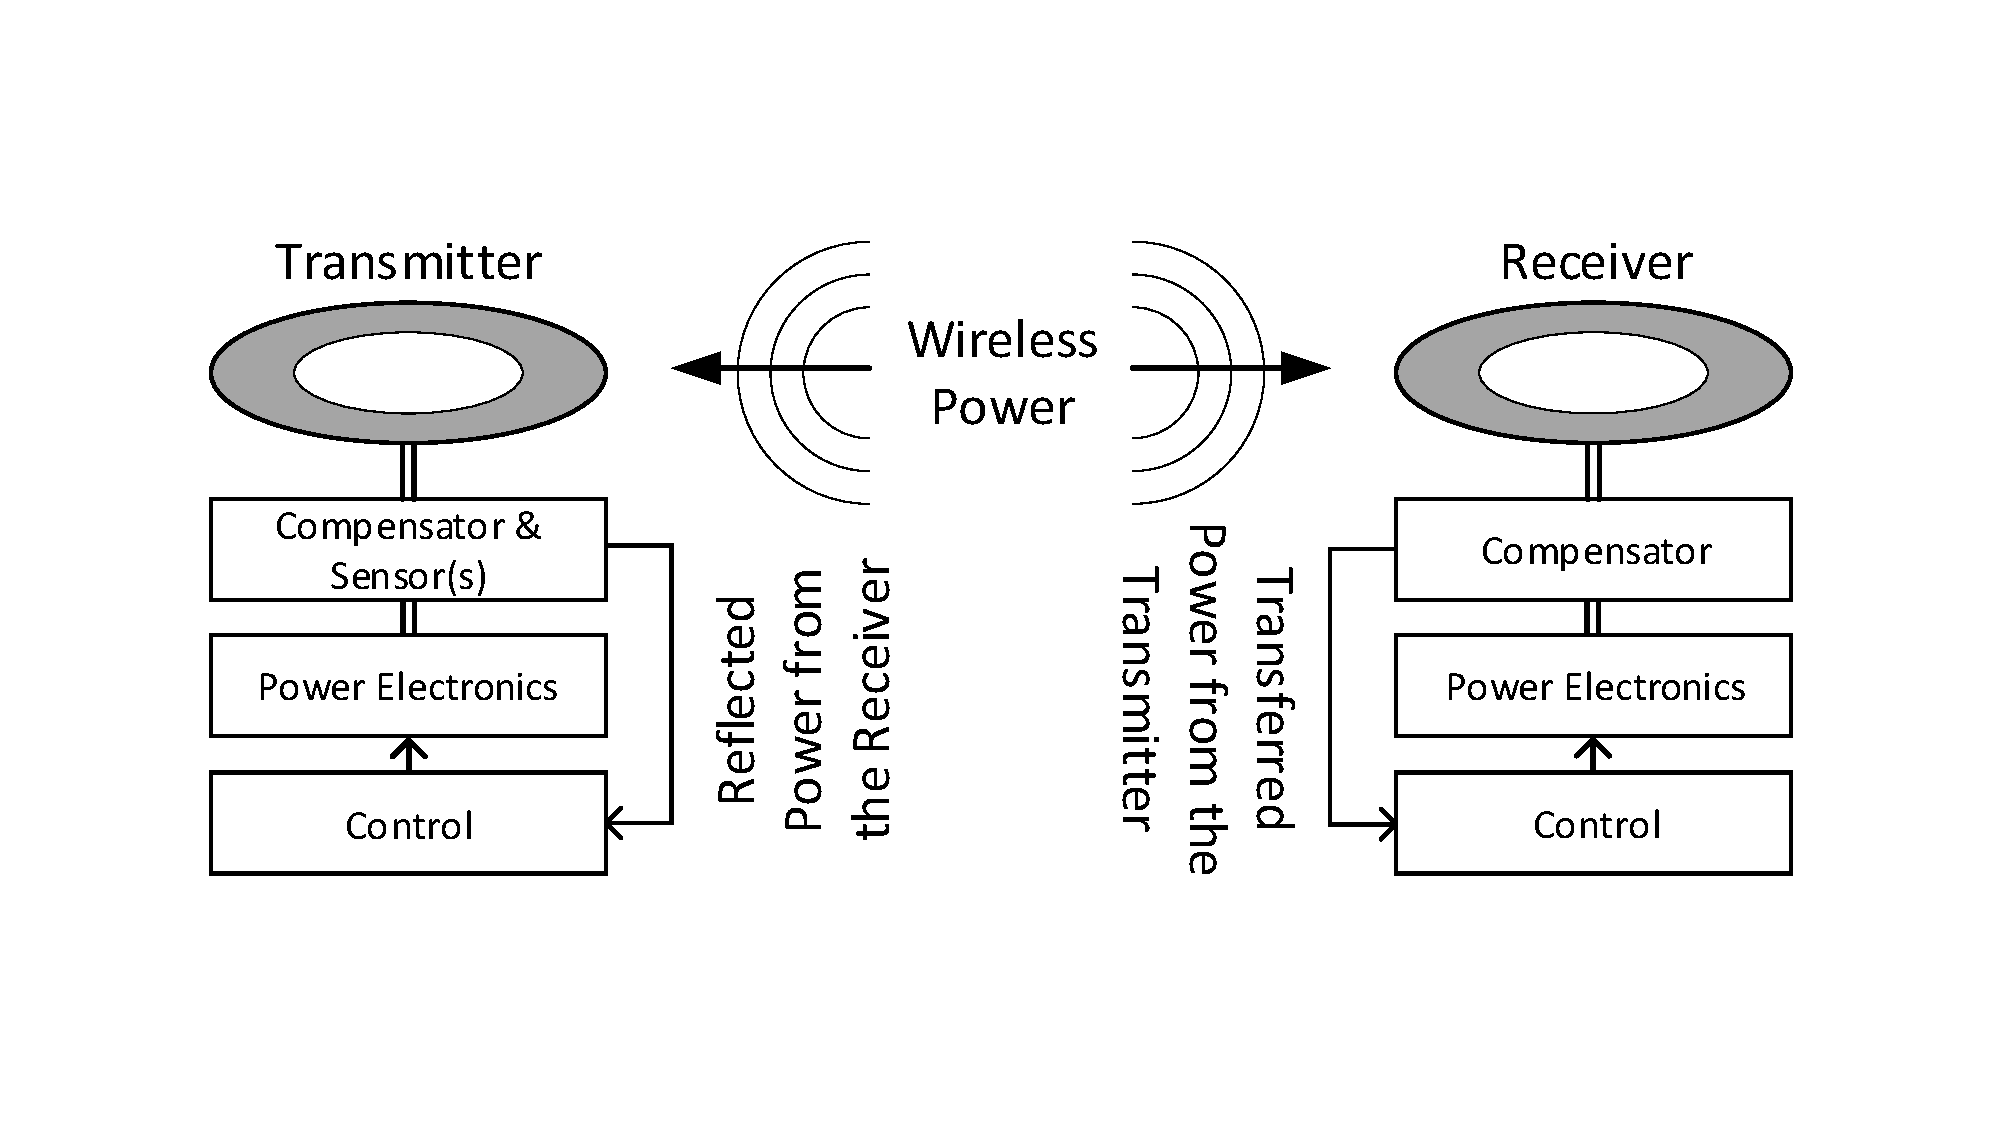
\includegraphics[clip, trim=0cm 3cm 0cm 3cm, width=1\columnwidth]{Figs/Fig1_c.pdf}
%        \vspace{-6mm}
    }%\vspace{-3mm}
    \caption{Different techniques in wireless identification of WPT coils; (a) indirect, (b) direct transmissive, and (c) direct reflective approaches.
    }
    \label{Fig1}
    \vspace{-6mm}
\end{figure}
In addition to the aforementioned system level studies, identification of the coupled side parameters and controlling the flow of power between them can be considered as one of the most important key concepts.
{\color{black} For instance, in dynamic WPT where electric vehicles are charged dynamically, the utility needs to meter the transferred power (energy) to charge the consumer according to the available energy tariff \cite{CHARGE1,CHARGE2}. Fast techniques of transferred power estimation is essential to control the transferred power to the moving receiver and to enhance the dynamics of the receiver circuitry \cite{ PC1, PC2}. For this purpose, transmitter senses and controls the power so that the received power is smooth and levelled when the moving receiver interacts with the transmitter pad. Hence, the proposed PWM-synchronized sampling power estimation technique could provide an efficient way of transferred power estimation necessary for the effective control of the power transfer process.}

As power in WPT systems is transferred wirelessly, the information flow between such coils must be carried out without any physical connection.
%\st{Although all of the aforementioned aspects are of the main building blocks in the structure of WPT systems, identification of the coupled side parameters and controlling the flow of power between them can be considered as one of the most important key concepts.} 
%{\color{red}These systems are designed not to have any physical connection.}
{\color{black}Therefore, wireless sensing of variables is introduced as a measure of identification of unknown parameters.}
%\st{Therefore, sensing each side is preferred to be done wirelessly from the coupled side.} 
The wireless sensing techniques can be categorized into two basic types, namely indirect and direct methods, as shown in Fig.~\ref{Fig1}. In the indirect approach, WPT sides communicate through additional wireless sensing techniques (for example, using techniques such as image processing \cite{IMAGE_RECOGNITION}, global positioning system (GPS) \cite{GPS_DETECTION_1, GPS_DETECTION_2}, infrared signal \cite{INFRARED}, ultrasonic signal \cite{ULTRASONIC}, or wireless power signal \cite{WPT_SENSE_1}), as shown in Fig.~\ref{Fig1}(a). Although some of these sensing techniques are extensively used in different applications such as position detection, they cannot be directly used to sense the WPT variables such as the profile of transferred power for controlling purposes. To sense the transferred power profile, the sensing needs to be done in the realm of WPT, and the sensing pads need to create an inductance profile (mutual inductance and self-inductance) similar to the main WPT pads. However, sensing and power coils may not create identical inductance profiles and that can lead to an inaccurate estimation. The other problem that may occur as a result of using indirect identification is the delay in response. 

On the other hand, in direct approach, WPT coil measurements are directly used for identification. This can be done transmissively, by sensing the power transferred from one side and received from the other side, as shown in Fig.\ref{Fig1}(b), or reflectively, by measuring the transferred power from one side and sniffing its reflection at the same (transmitting) side, as shown in Fig.\ref{Fig1}(c). Identification in the reflective direct techniques can be carried out by observing the amplitude of the influenced (reflected) signal \cite{HAN_AMPL_REF,ZHAO_AMPL_REF} or its frequency content \cite{LUSI_FRQ_REF, LI_FRQ_REF, KHAL_FRQ_REF}. The sensing can be carried out Interruptedly or continuously. In the first approach of the interrupted cycles of sensing, the WPT process is to be halted for a short period of time to identify the receiver parameters. In this direct approach, although the same WPT transmitter is used to sense the receiver, sensing interruptions can decrease the overall transferred power and it can create some undesirable transients in the transmitter side \cite{LUSI_FRQ_REF, LI_FRQ_REF, KHAL_FRQ_REF}. Therefore, continuous techniques are proposed to observe the receiver through the same WPT transmitter with a minimum influence on the WPT process \cite{HAN_AMPL_REF,ZHAO_AMPL_REF}. As a result, direct approaches are more reasonable to sense the flow of the transferred power.
Different combinations of all these techniques can be used to extract more information from the wirelessly coupled coils. These techniques can effectively estimate the reflected impedance of the receiver coil seen from the transmitter coil. Although in some articles, the \mathit{estimation of mutual inductance} is the topic of concern, without knowing the load information of the far-end coil, the estimation of mutual inductance is not possible. Therefore, another communication link or  predetermined load information is needed for the estimation of mutual inductance.

In this article, by sampling of the LCC parallel capacitor voltage in the WPT system shown in Fig.~\ref{Fig.Fig2}, the transferred power to the receiver is estimated. A novel approach of PWM-synchronized sampling is used to estimate the transferred power. The studies are carried out by defining a new criterion termed as demand factor. To elaborate this technique, Section II describes how the transferred power can be estimated from a transmitter equipped with an LCC network. Section III is dedicated to analyze the influence of the detuned reactances on the operation of the proposed system. In Section IV, the influence of stray series resistances on the estimation is analyzed, and finally Section V compares the numerical and experimental results to prove the validity of the proposed approach.
%% FIG2
\begin{figure}[t]
%\vspace{-5mm}
\centerline{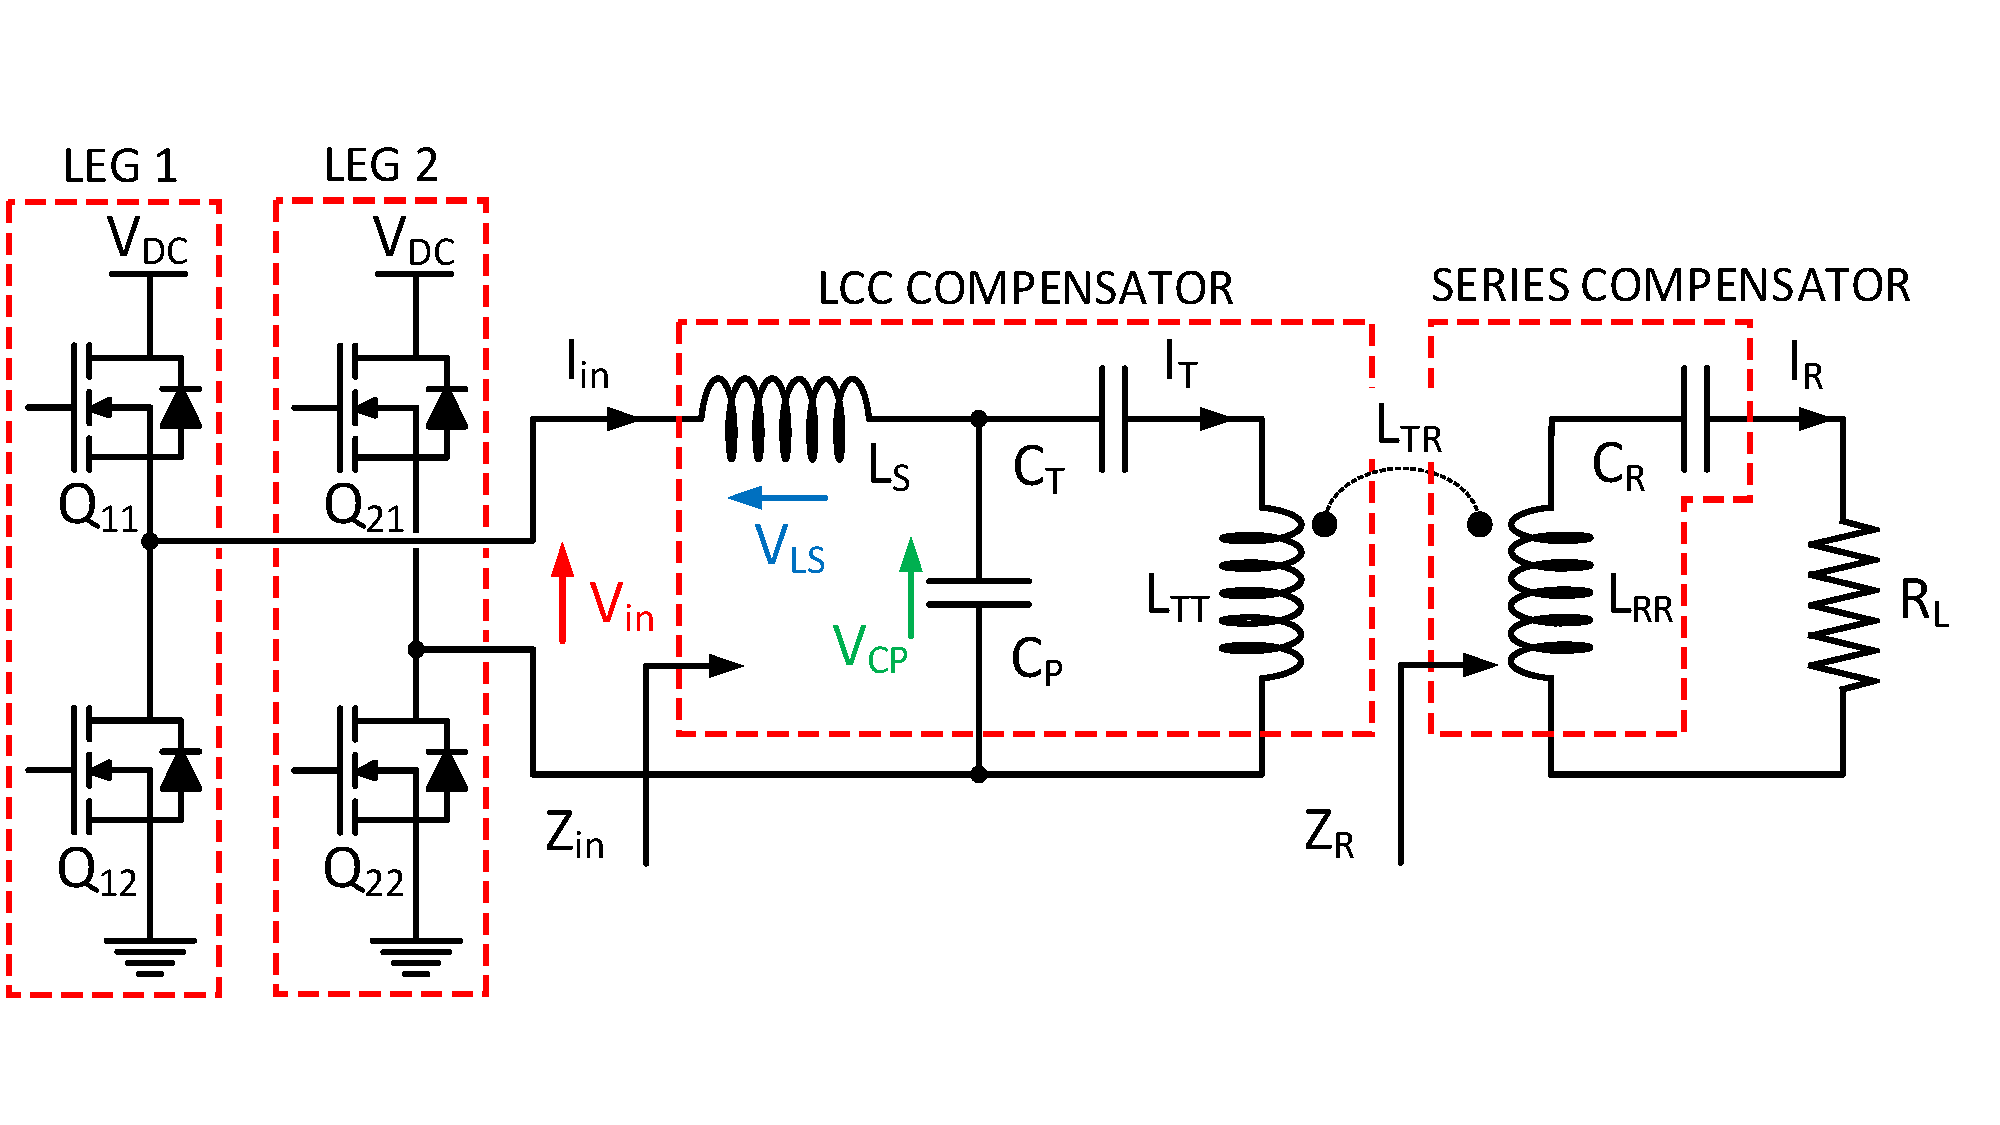
\includegraphics[clip, trim=0cm 2cm 0cm 2cm, width=1\columnwidth]{Figs/Fig2.pdf}}
\caption{Circuit diagram of a WPT system equipped with an LCC and series capacitor in transmitter and receiver coils respectively.}
\vspace{-3mm}
\label{Fig.Fig2}
\end{figure}
%% FIG3
\begin{figure}[t]
	\centerline{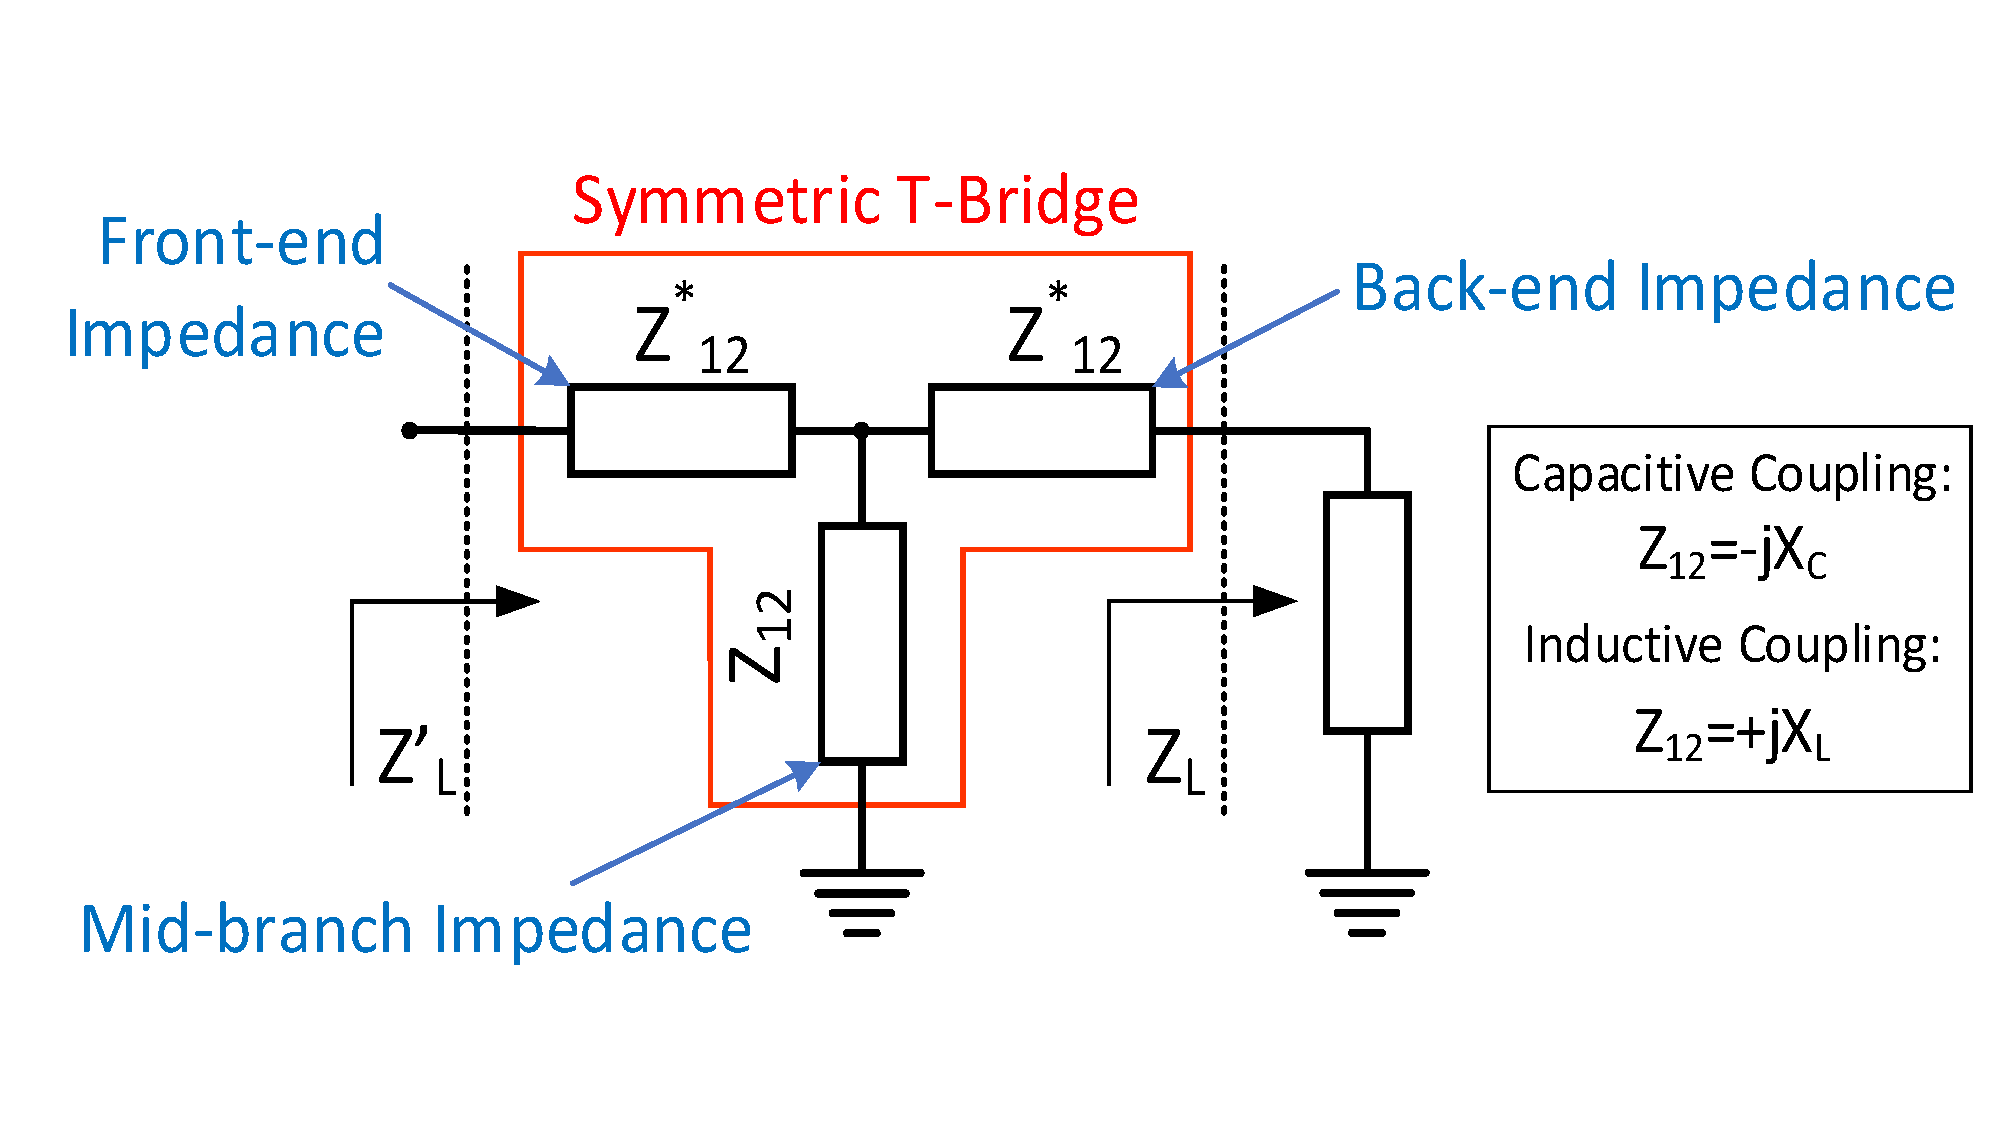
\includegraphics[clip, trim=0cm 1cm 0cm 1cm, width=0.8\columnwidth]{Figs/Fig3.pdf}}
	\vspace{-3mm}
	\caption{Symmetric T-Bridge.}
	\label{Fig.Fig3}
	\vspace{-3mm}
\end{figure}
%%
\section{Operation Principles of the System}
In this section, how the variation of mutual inductance influences the transmitter LCC compensator will be investigated. For this purpose, the reflection of the load impedance in a symmetric T-Bridge is explained. Then, using this concept, it is shown how the receiver load will be seen from the transmitter LCC input terminals.
%%
\subsection{Symmetric T-Bridge}
Symmetric T-Bridge is considered as a passive T-shape LC network, as shown in Fig.~\ref{Fig.Fig3}. It has identical magnitude of {\color{black} reactance} in all its branches with the front-end and back-end impedances being complex conjugate of the mid-branch impedance. This configuration can be repeatedly seen in different places of WPT systems, such as coupled inductors and LCC compensators. Therefore, characterizing its operation will make the analysis of WPT systems easier.
For this bridge, the load impedance $Z_{\rm L}$ seen from the input terminals of the bridge $Z'_{\rm L}$ is given in \eqref{EQ.EQ.1}.
%%EQ1
\begin{flalign}
\label{EQ.EQ.1}
Z'_{\rm L}&=|Z_{12}|^2/Z_{\rm L}=X_{\mathrm{C}/\mathrm{L}}^2/Z_{\mathrm{L}} &
\end{flalign}
%%%

\subsection{Measuring the Demand Factor in an LCC Compensator}
%% FIG4
\begin{figure}[t]
	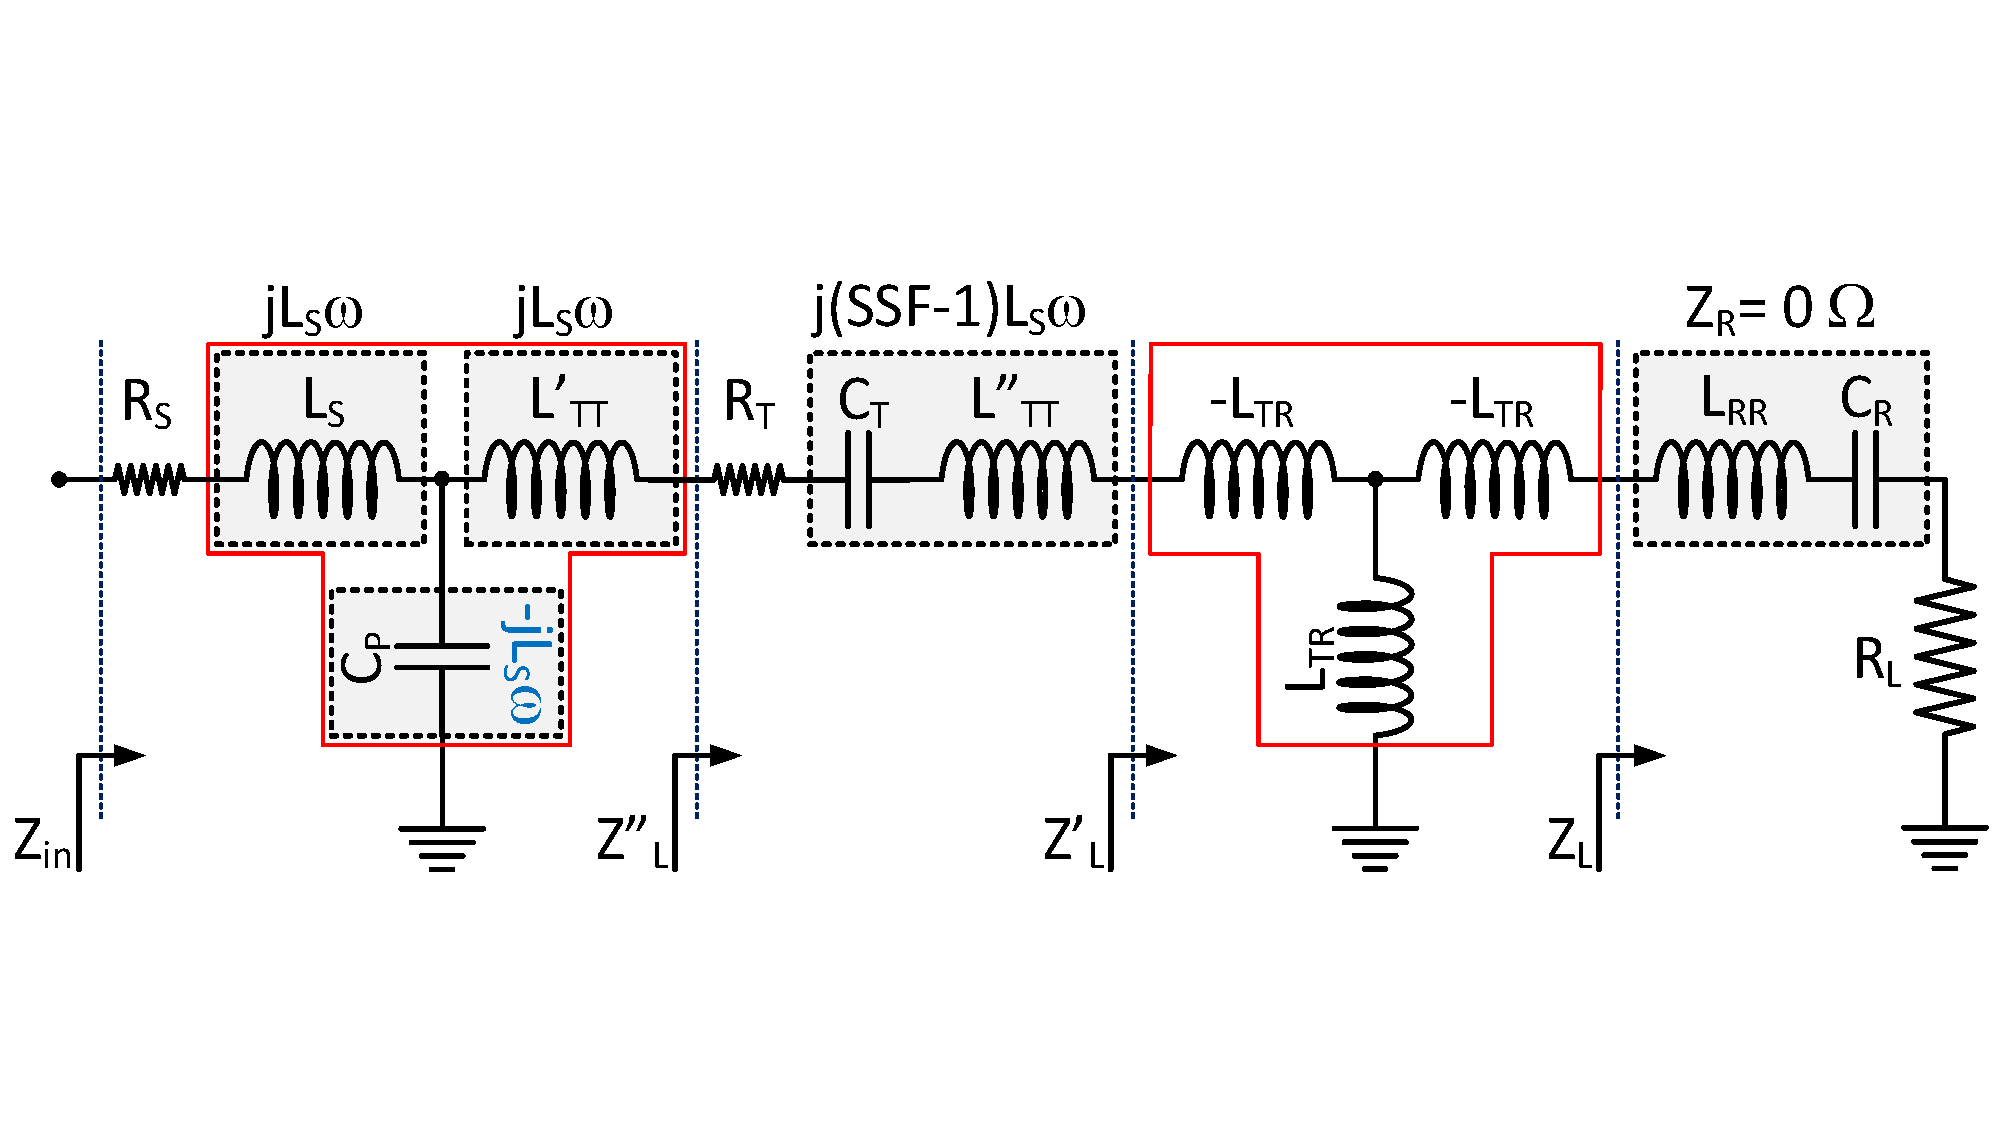
\includegraphics[clip, trim=0.3cm 4cm 0cm 4cm, width=1\columnwidth]{Figs/Fig4.pdf}
	\caption{Equivalent circuit of the LCC-S compensated WPT system indicating impedances at different stages.}
    \label{Fig.Fig4}
    \vspace{-3mm}
\end{figure}
%%
The proposed WPT system shown in Fig.~\ref{Fig.Fig2} can be rearranged to form a cascaded symmetric T-bridge network as shown in Fig.~\ref{Fig.Fig4}. In this circuit, transmitter self-inductance $L_{\rm TT}$ is divided into two parts $L'_{\rm TT}=L_{\rm S}$ and $L''_{\rm TT} =L_{\rm TT}-L_{\rm S}$ to make the symmetric T-bridges visible in the equivalent circuit. The component values, including the front-end inductance, the coil inductances, and the compensation capacitors, are chosen to comply with the following relation at the operating frequency of $\omega$.
%% EQ2
\begin{flalign}
    \omega  =\dfrac{1}{\sqrt{L_{\rm S} C_{\rm P} }} = \dfrac{1}{\sqrt{L'_{\rm TT} C_{\rm P} }}     = \dfrac{1}{\sqrt{L_{\rm RR} C_{\rm R} }}   &&  
    \label{EQ.Freq_relations}
\end{flalign}
%%
\noindent To achieve a desirable level of soft-switching,
%% EQ3
\begin{flalign}
    ({K_{\mathrm{SSF}}} -1)\omega L_{\rm S}    = \omega     L''_{\rm TT} -\frac{1}{\omega C_{\rm T}} &&
\end{flalign}
%%
\noindent where $\omega$ is the fundamental frequency of the source and {\color{black}$K_{\mathrm{SSF}}$ is the Soft-Switching Factor of the LCC Network. This factor is unity for zero phase switching (when the fundamental of $v_\mathrm{in}$ has the same phase angle with $i_\mathrm{in}$) and is equal to $\pi^2/8$ for zero current switching \cite{Pantic} (when $i_\mathrm{in}$ is zero at the zero crossing moments of $v_\mathrm{in}$)}. Next, in order to simplify the analysis, parasitic resistances of all the components, such as equivalent series resistances (ESRs) of $L_{\mathrm{S}}$ and power supply ($R_{\mathrm{S}}$) and transmitter ($R_{\mathrm{T}}$) are assumed to be negligibly small and are approximated to zero for the subsequent analyses. The input impedance seen from the input of the LCC network $Z_{{\rm in}}$ at the operating frequency $\omega$ can be derived from \eqref{EQ.EQ.2}.
%% EQ4
\begin{flalign}
\label{EQ.EQ.2}
    Z_{{\rm in}}=\dfrac{L_{\rm S}^2\omega^2}{\dfrac{L_{\rm TR}^2\omega^2}{R_{\rm L}}+{\rm j }(K_{\mathrm{SSF}}-1)L_{\rm S}\omega} &&
\end{flalign}
%%
\noindent where $R_{\rm L}$ is  the load resistance. {\color{black}From \eqref{EQ.EQ.2} it can be seen that $Z_\mathrm{in}$ is capacitive for $K_\mathrm{SSF}>1$, and it is inductive for $K_\mathrm{SSF}<1$. It is also clear that $Z_\mathrm{in}$ is resistive for $K_\mathrm{SSF}=1$, and it makes $i_\mathrm{in}$ have the same phase angle with the fundamental of $v_\mathrm{in}$. However, as $v_\mathrm{in}$ is a rectangular waveform, some capacitive $Z_\mathrm{in}$ is needed to maintain the zero current switching. The optimized capacitive behavior for zero current switching when the system is fed by a rectangular waveform is $K_\mathrm{SSF}=\pi^2/8$ \cite{Pantic}.} The injected apparent power to the LCC compensator at the fundamental frequency $\omega$ can be obtained from \eqref{EQ.EQ.3}.
%% EQ5
\begin{flalign}
    S_{\rm in}= 
    \frac{|V_{\rm in}|^2}{Z_{\rm in}} = 
    {\underbrace{
    \overbrace{
    \left(
    \frac{L_{\rm TR}^2\omega^2}{R_{\rm  L}}
    \right)
    }^{\xi}
    \frac{1}{L_{\rm S}^2\omega^2}|V_{\rm in}|^2}_\text{Active Power}
    -{\rm j}
    \underbrace{\frac{K_{\mathrm{SSF}}-1}{L_{\rm S}\omega}|V_{\rm  in}|^2}_\text{Reactive Power}}&&
\label{EQ.EQ.3}
\end{flalign}
%%
\noindent which includes active power and reactive power components.
On the other hand, as the primary (front-end) loop of the LCC compensator is fully compensated, it acts as a current source for the transmitter current $I_{\textrm T}$, which is equal to $-{\textrm{j}C_{\textrm{P}}}\omega V_{\rm in}$. Therefore, receiver current $I_{\rm R}$ is equal to $\left({L_{\rm TR}}/{L_{\rm S}}\right)V_{\rm in}$, and the transferred power (output power)  ($P_{\rm out}$) can be derived from the following equation.
%% EQ6
\begin{flalign}
    P_{\rm out}=R_{\rm L}|I_{\rm R}|^2=\overbrace{
    \bigg(\frac{L_{\rm TR}^2\omega^2}{R_{\rm L}}\bigg)}^{\xi}
    \frac{1}{L_{\rm S}^2\omega^2}|V_{\rm in}|^2
    =\frac{\xi}{L_{\mathrm{S}}^2\omega^2}\left|V_{\rm in}\right|^2 &&
\label{EQ.EQ.4}
\end{flalign}
%%Fig5
\begin{figure}[t!]
\begin{center}
	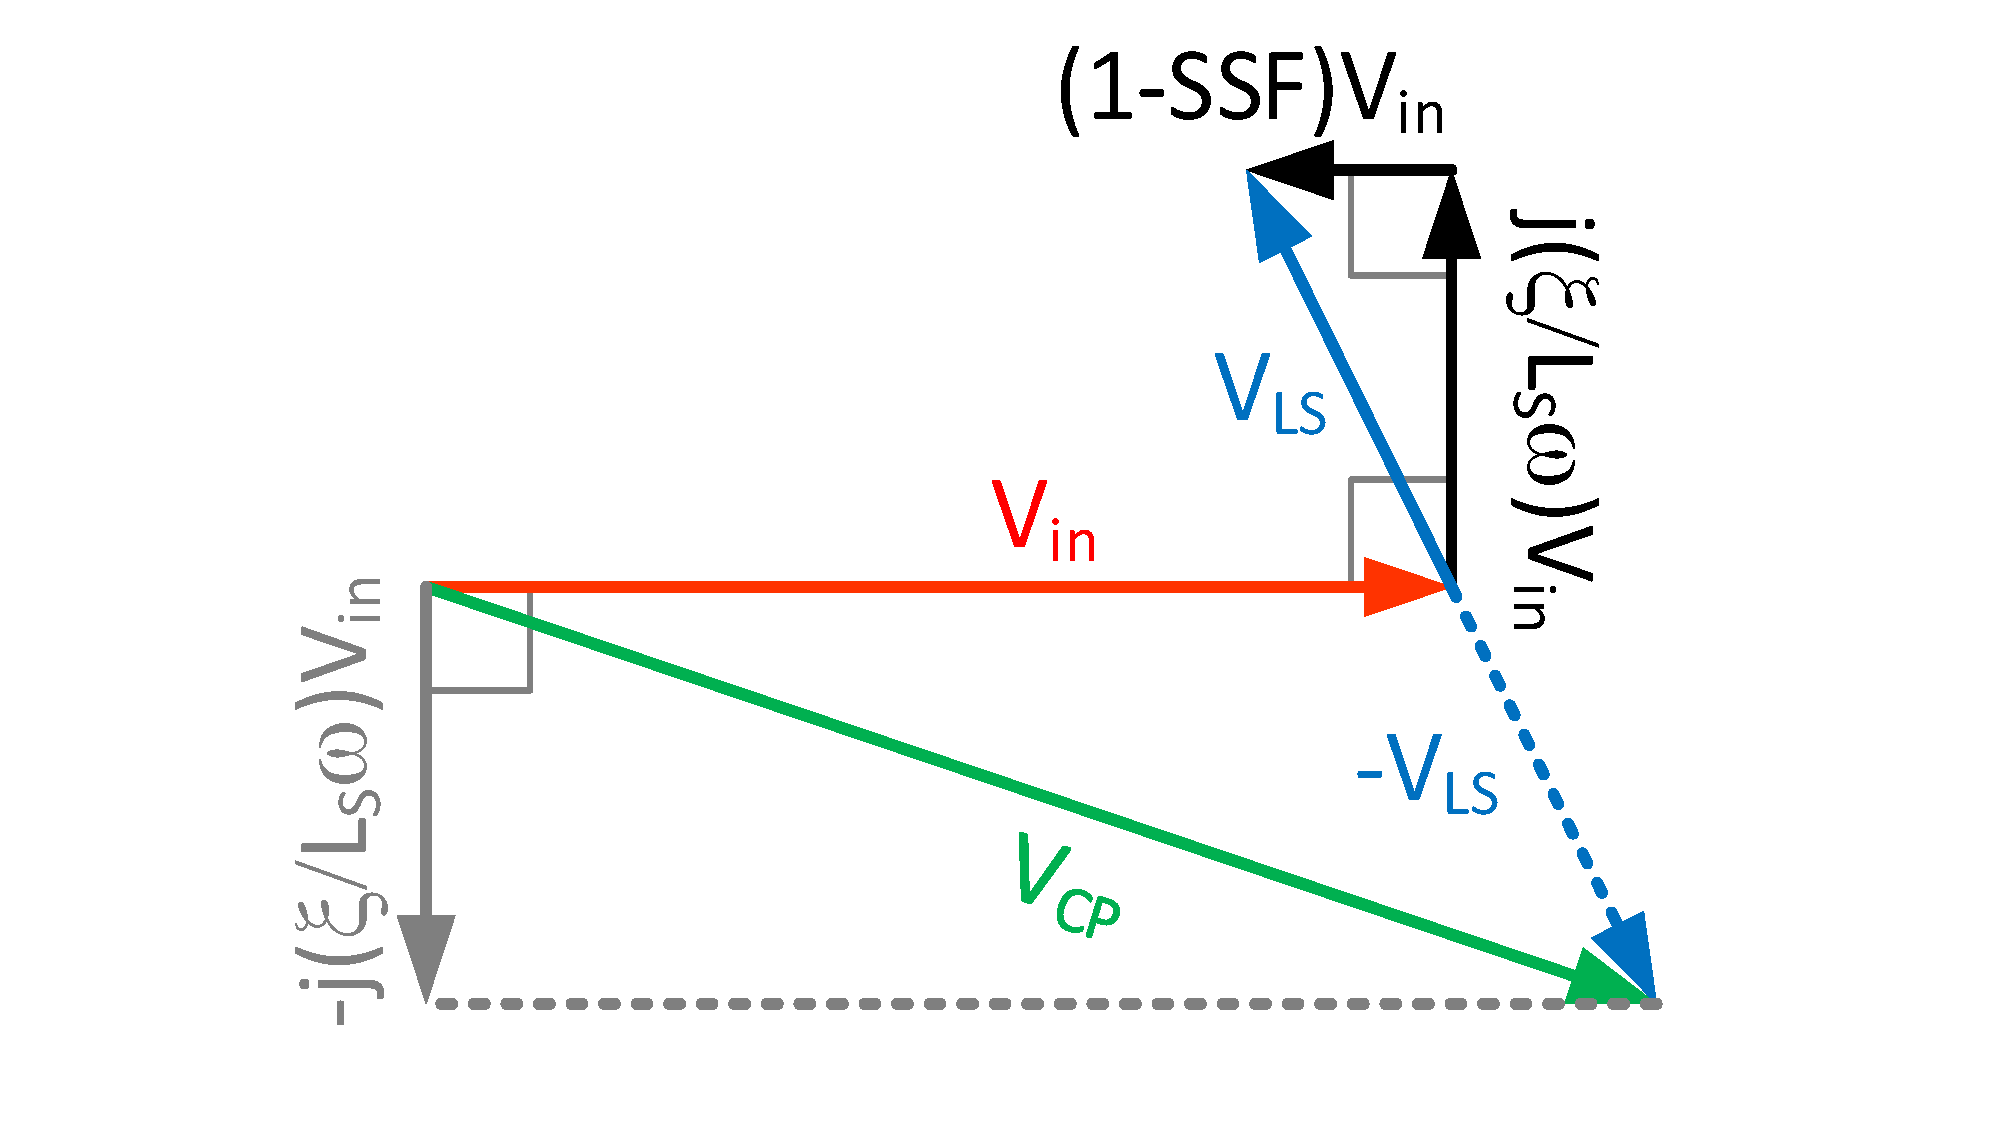
\includegraphics[clip, trim=0cm 0cm 0cm 0cm, width=.65\columnwidth]{Figs/Fig5.pdf}
\end{center}
\vspace{-0.2cm}
	\caption{$V_\textrm{LS}$ and $V_\textrm{CP}$ phasors of the LCC front-end signals.}
		\label{Fig.Fig5}
		\vspace{-3mm}
\end{figure}
It is interesting to observe from  \eqref{EQ.EQ.3} and \eqref{EQ.EQ.4} that under the assumption of lossless components, the active power component in $S_{\rm in}$ is equal to the output active power consumed by the load, and the reactive power component of $S_{\rm in}$ does not depend on the transmitter-receiver mutual inductance and receiver parameters. However, the active power is also dependent on the receiver load $R_\mathrm{L}$ and the transmitter-receiver mutual inductance $L_\textrm{TR}$ through ${L_{\textrm{TR}}^2\omega^2}/{R_\textrm{L}}$. Therefore, the term ${L_{\textrm{TR}}^2\omega^2}/{R_\textrm{L}}$, which makes a direct relationship between the input and output powers and depends on the receiver parameters, is defined as the demand factor $\xi$. In LCC networks, this factor is equal to the reflected impedance $Z'_{\mathrm{L}}$; however, it is different for other types of compensators. $\xi$ can be estimated by directly measuring the active power from the LCC front-end terminals. In fact, with the assumption of loss-less ideal components, this is the expected phenomenon as input active power is completely consumed by the receiver load. Nevertheless, this principle can still be exploited even in a practical scenario (when the ESRs are present) to estimate and control the output power as long as the quality factor of the transmitter circuitry is kept high.

Therefore, in order to estimate the output power requirement, one does not need to estimate both mutual inductance and the load impedance. Instead, the transferred power can be directly calculated by estimating $\xi$. For this purpose, $\xi$ can be identified by measuring the fundamental voltage component of the LCC front-end elements of $L_{\mathrm{S}}$ or $C_{\mathrm{P}}$, $V_\textrm{LS}$ or $V_\textrm{CP}$, which are given in \eqref{EQ.EQ.7} and \eqref{EQ.EQ.8}, respectively. According to \eqref{EQ.EQ.7} and \eqref{EQ.EQ.8}, the quadrature component of these voltages is proportional to the demand factor, which makes $V_\textrm{LS}$ and $V_\textrm{CP}$ excellent measurement candidates for the estimation of the demand factor. In case of zero phase switching, $K_{\mathrm{SSF}}=1$, $V_\textrm{LS}$ is completely proportional to the demand factor. Nevertheless, zero phase switching may not be preferable due to the switching concerns \cite{Pantic}. In that case, the quadrature component of the measured $V_\textrm{LS}$ or $V_\textrm{CP}$ with reference to $V_\textrm{\rm in}$ needs to be obtained, as illustrated in Fig.~\ref{Fig.Fig5}.
%%EQ7
\begin{flalign}
    V_{\rm LS}=(1-K_{\mathrm{SSF}})V_{\rm in}+{\rm j}\left(\frac{\xi}{L_{\rm S}\omega}\right)V_{\rm in} &&
    \label{EQ.EQ.7}
\end{flalign}
%%
%%EQ8
\begin{flalign}
    V_{\rm CP}=V_{\rm in}-V_{\rm LS}=(K_{\mathrm{SSF}})V_{\rm in}-{\rm j}\left(\frac{\xi}{L_{\rm S}\omega}\right)V_{\rm in} &&
    \label{EQ.EQ.8}
\end{flalign}
%%


%% FIG6
\begin{figure}[t!]
\begin{center}
	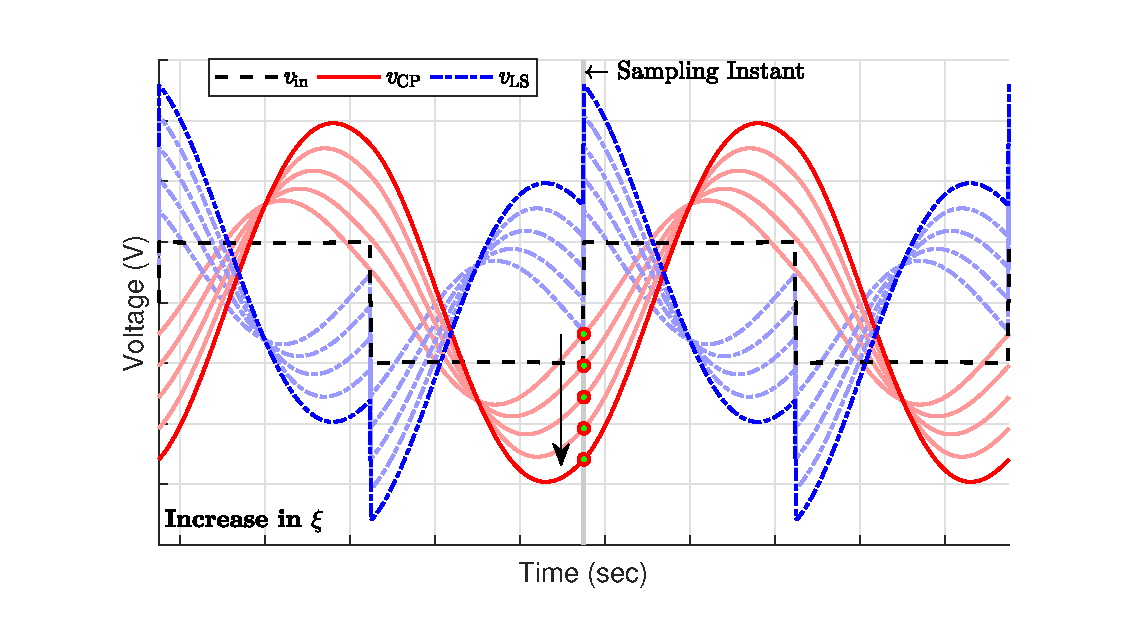
\includegraphics[clip, trim=1cm 0.0cm 1cm 0.0cm, width=1\columnwidth]{Figs/Fig6.eps}
\end{center}
\vspace{-0.2cm}
	\caption{$v_\textrm{\rm in}$, $v_\textrm{CP}$, and $v_\textrm{LS}$ LCC front-end wave-forms of voltage, and variation of $v_\textrm{CP}$ PWM-synchronized samples with the changes in $\xi$.}
		\label{Fig.Fig6}
		\vspace{-3mm}
\end{figure}
%%
Fig.~\ref{Fig.Fig5} shows that the quadrature components of $V_{\rm LS}$ and $V_{\rm CP}$ have the same amplitude, but they are $180^\circ$ out of phase. However, this assumption is only valid when there are no other harmonics except the fundamental frequency. Therefore the following subsection, analyses a more realistic implementation by considering the effects of higher-order harmonics. 
\subsection{Harmonic Analysis}
Practically, the WPT system is driven by a rectangular waveform of voltage as shown in Fig.~\ref{Fig.Fig6}. Using the Fourier analysis, the simplified equivalent circuit for the $n^{\rm th}$ harmonic is shown in Fig.~\ref{Fig.Fig7}, and neglecting the effect of LCC back-end branch for harmonics, the voltage across $L_{\mathrm{S}}$ and $C_{\mathrm{P}}$ can be determined as given in \eqref{EQ.EQ.9} and \eqref{EQ.EQ.10} \cite{Pantic}.
%% FIG7
\begin{figure}[t!]
\begin{center}
	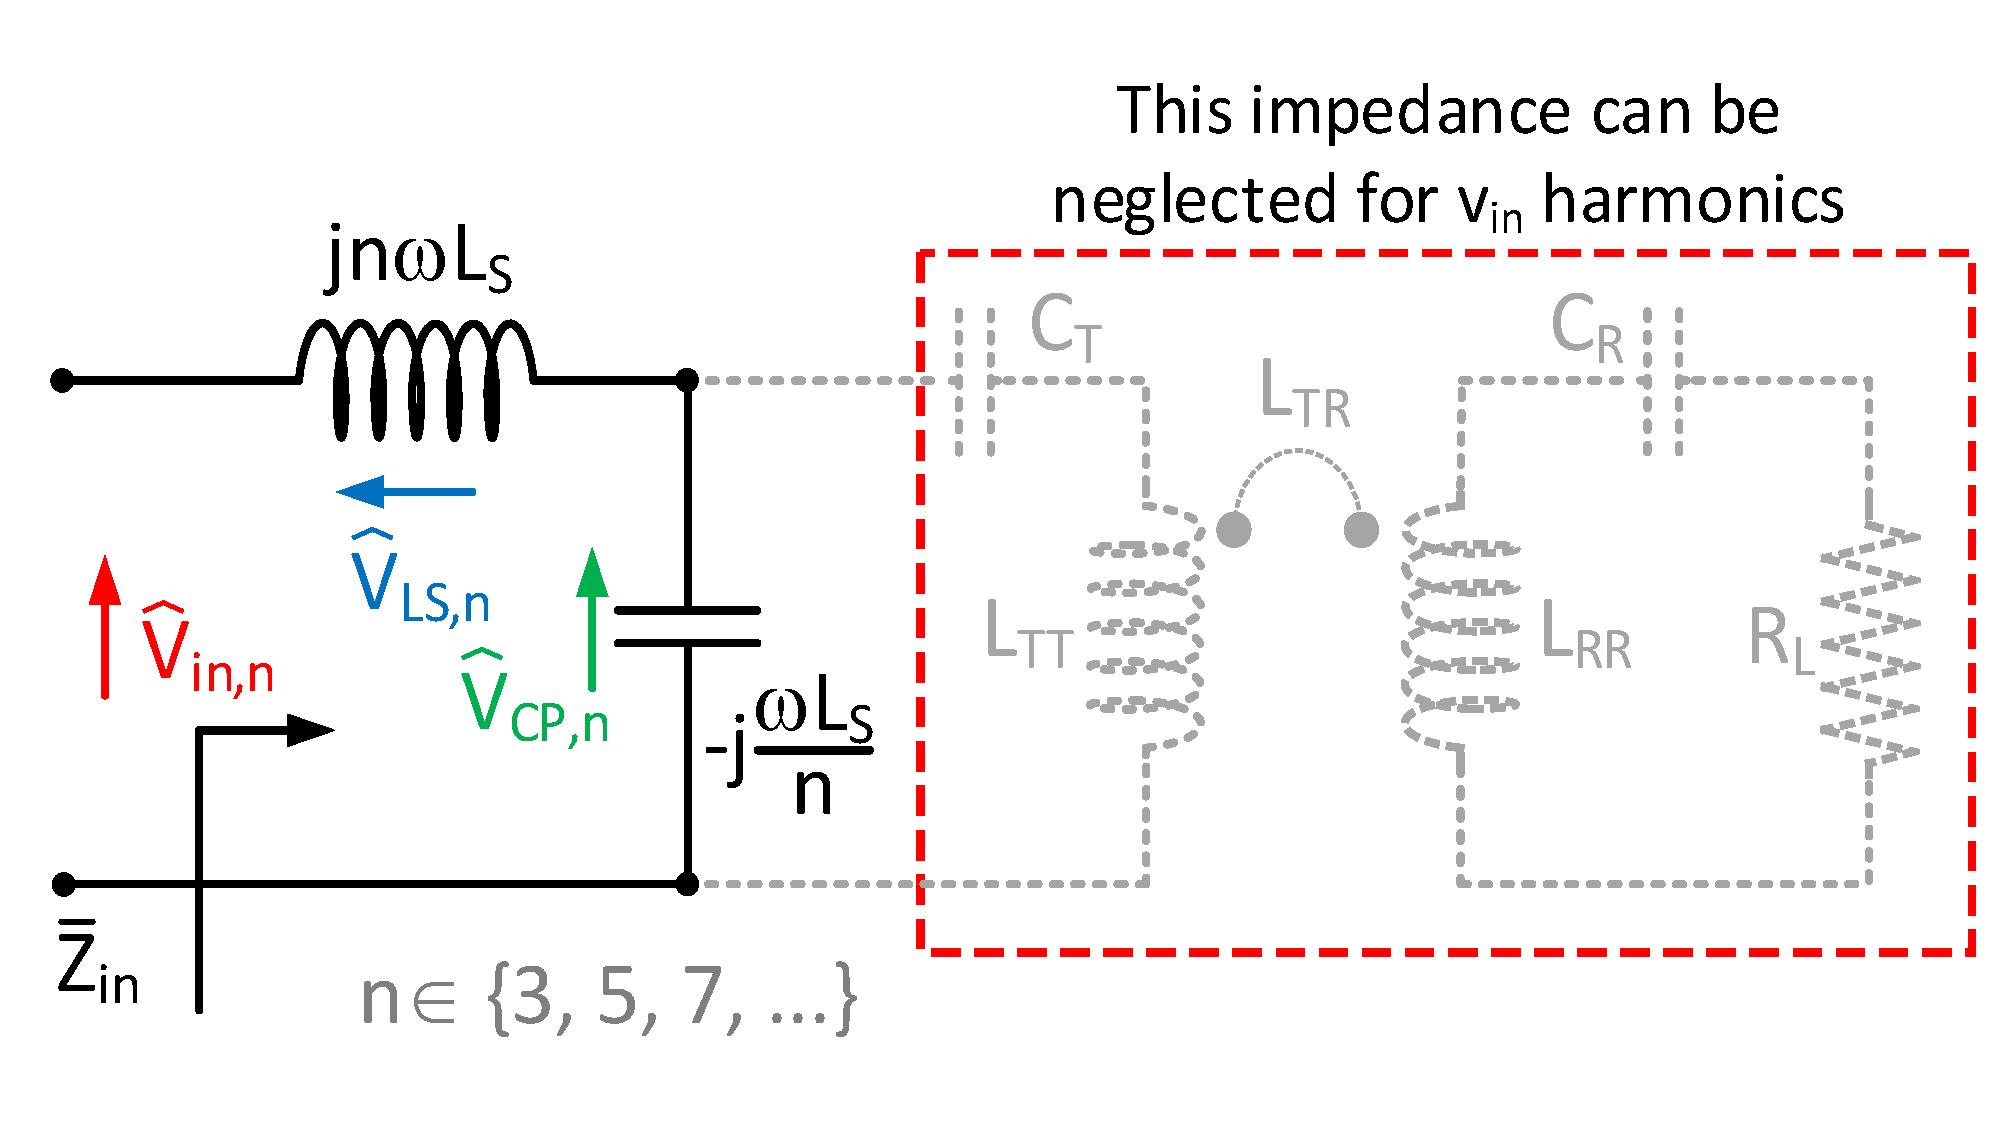
\includegraphics[clip, trim=0cm 1cm 0cm 1cm, width=0.75\columnwidth]{Figs/Fig7.pdf}
\end{center}
\vspace{-0.2cm}
	\caption{Simplified circuit of the transmitter circuitry for harmonic contents.}
		\label{Fig.Fig7}
		\vspace{-5mm}
\end{figure}
%% EQ9
\begin{flalign}
    \bar{v}_{\textrm{LS}}=\frac{4V_{\textrm{DC}}}{\pi}\sum\limits^{\infty}_{n=3, 5, ...}{\overbrace{\frac{n}{n^2-1}}^{\hat{V}_{\mathrm{LS},n}}\sin{\left(n\omega t\right)}} &&
    \label{EQ.EQ.9}
\end{flalign}
%% EQ10
\begin{flalign}
    \bar{v}_{\textrm{CP}}=-\frac{4V_{\textrm{DC}}}{\pi}\sum\limits^{\infty}_{n=3, 5, ...}{\overbrace{\frac{1}{n\left(n^2-1\right)}}^{\hat{V}_{\mathrm{CP},n}}\sin{\left(n\omega t\right)}} &&
    \label{EQ.EQ.10}
\end{flalign}
%%
\noindent where $n$ is the harmonic order of the rectangular waveform of the input voltage $V_{\textrm{\rm in}}$ shown in Fig.~\ref{Fig.Fig6}, and $\bar{v}_{\textrm{LS}}$ and $\bar{v}_{\textrm{CP}}$ represent the harmonic content of the corresponding voltages. Comparing \eqref{EQ.EQ.9} and \eqref{EQ.EQ.10}, it is apparent that the influence of harmonics on $\hat{V}_{\textrm{LS},n}$ is $n^{2}$ times that of $\hat{V}_{\textrm{CP},n}$, which makes $V_{\textrm{CP}}$ less vulnerable to the harmonics. Therefore, $V_{\textrm{CP}}$ becomes a more viable candidate for direct estimation of $\xi$. This is especially important when the direct measurements are to be done to esitmate the transferred power.
To explain the PWM-Synchronized sampling, fundamental components of the input voltage and voltage $v_{\mathrm{CP}}(t)$ can be written as in  \eqref{EQA1} and \eqref{EQA2}.
%% EQ11
\begin{flalign}
    v_{\textrm{in}}=|V_{\mathrm{in}}|\sin(\omega t) &&
    \label{EQA1}
\end{flalign}
%% EQ12
\begin{flalign}
    v_{\textrm{CP}}=
    \overbrace{|V_{\mathrm{CP}}|\cos(\psi)}^{V_{\mathrm{CP},d}}\sin(\omega t)
    +
    \overbrace{|V_{\mathrm{CP}}|\sin(\psi)}^{V_{\mathrm{CP},q}}\cos(\omega t) &&
    \label{EQA2}
\end{flalign}
%%
\nonindent where $\psi$ is the phase angle between $V_{\mathrm{CP}}$ and $V_{\mathrm{in}}$ and $k \in \mathbb{Z}$ is the sampling index. Therefore, the quadrature component of the LCC parallel capacitor $V_{\mathrm{CP},q}$, can be achieved as follows.
%% EQ13
\begin{flalign}
    V_{\textrm{CP},q}(k)=v_{\textrm{CP}}(\omega t);~~~~\omega t = (2k+1)\frac{\pi}{2} &&
    \label{EQA3}
\end{flalign}
%%
Equation \eqref{EQA3} explains how by taking samples from $v_\mathrm{CP}$ at the moments of input voltage $v_{\rm in}$ zero crossing, the quadrature component of the front-end ($V_{\mathrm{CP}}$) is achievable. $V_{\mathrm{CP},q}$ samples for different demand factors are shown as the circled markers at the input voltage zero crossing sampling instant shown in Fig.\ref{Fig.Fig6}. Therefore, from equations \eqref{EQ.EQ.8} and \eqref{EQA3}, the transferred power $P_\mathrm{out}$ {\color{black}for negligible $R_\mathrm{S}$ and $R_\mathrm{T}$} can be estimated by only taking PWM-Synchronized samples from $v_{\mathrm{CP}}$ and calculating the input power ($P_{\mathrm{in}}$) as elaborated in $\eqref{EQA4}$.
%% EQ14
\begin{flalign}
    P_{\mathrm{out}}(k)\approx P_{\textrm{in}}(k)=\frac{2}{\pi}\frac{V_{\mathrm{DC}}}{L_\mathrm{S}\omega}\left|V_{\textrm{CP},q}(k)\right| &&
    \label{EQA4}
\end{flalign}
%%
\noindent where $V_{\mathrm{DC}}$ is the DC-link voltage of the resonant converter shown in Fig.~\ref{Fig.Fig2}.

\section{Influence of the Detuned Reactances}
In this section, the effect of detuning, which can happen in a practical situation is analyzed. To this end, it is assumed that the front-end loop of the LCC network, back-end loop of the LCC network, and series compensated receiver are not properly tuned, and they are detuned by $\Delta X_\mathrm{S}$, $\Delta X_\mathrm{T}$, and $\Delta X_\mathrm{R}$ respectively. ESRs of the network are also considered negligible to simplify the calculations. Therefore, having the detuned reactances, the equivalent circuit diagram of the system is obtained as shown in Fig.~\ref{FigA1}.
\begin{figure}[t]
	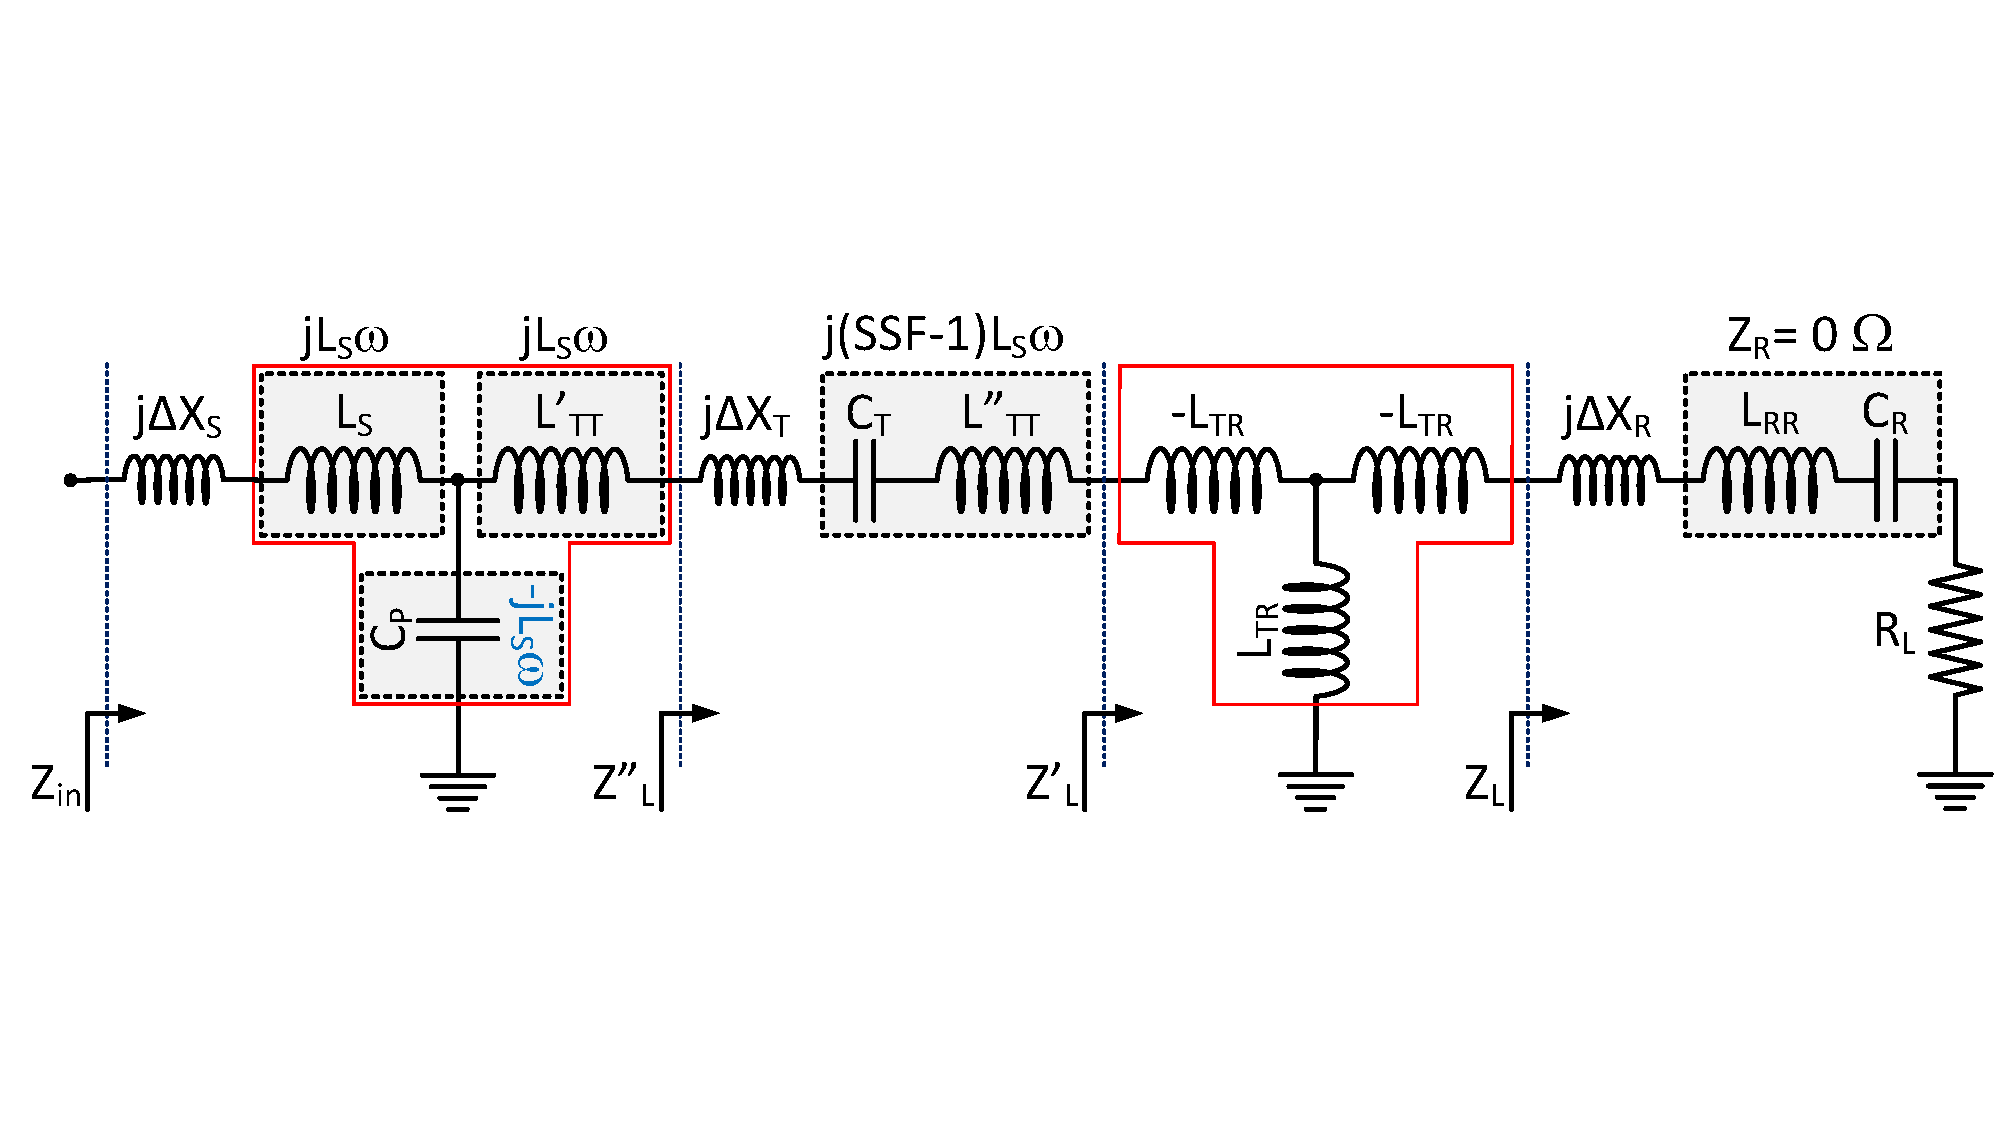
\includegraphics[clip, trim=0.3cm 5cm 0cm 5cm, width=1\columnwidth]{Figs/FigA1.pdf}
	\caption{Equivalent circuit of the proposed WPT system with detuned reactances.}
    \label{FigA1}
    \vspace{-3mm}
\end{figure}
In the first step, it is assumed that only receiver is detuned by $\Delta X_\mathrm{R}$. This assumption changes equation \eqref{EQ.EQ.3} to \eqref{EQB1}.
%% EQ15
\begin{flalign}
    S_{\mathrm{in}} = 
    \underbrace{
    \frac{\xi_\mathrm{R}}{L_\mathrm{S}^2\omega^2}
    \left|V_{\mathrm{in}}\right|^2
    }_\text{Active Power}
    %  &&
    % \nonumber
% \end{flalign}
% \vspace{-5mm}
% \begin{flalign}
    +\mathrm{j}
    \underbrace{
    \left(
    -
    \frac{\xi_\mathrm{I}}{L_\mathrm{S}^2\omega^2}
    +
    \frac{K_{\mathrm{SSF}}-1}{L_\mathrm{S}\omega}
    \right)
    \left|V_{\mathrm{in}}\right|^2
    }_\text{Reactive Power}
     &&
    \label{EQB1}
\end{flalign}

\noindent where $\xi=\xi_{\mathrm{R}}-\mathrm{j}\xi_{\mathrm{I}}$ becomes a complex number due to the presence of ${\Delta X_\mathrm{R}}$. In \eqref{EQB1}, $\xi_\mathrm{R}=L_\mathrm{TR}^2\omega^2\left(
    \frac{R_\mathrm{L}}{R_\mathrm{L}^2+{\Delta X_\mathrm{R}}^2}
    \right)$ and $\xi_\mathrm{I}=L_\mathrm{TR}^2\omega^2\left(
    \frac{{\Delta X_\mathrm{R}}}{R_\mathrm{L}^2+{\Delta X_\mathrm{R}}^2}
    \right)$. Therefore, $V_\mathrm{CP}$ is changed to the following equation.
%% EQ16
\begin{flalign}
    V_{\mathrm{CP}} = 
    \overbrace{
    \left(K_{\mathrm{SSF}}-
    \frac{\xi_{\mathrm{I}}}{L_\mathrm{s}\omega}\right)V_{\mathrm{in}}
    }^{V_{\mathrm{CP},d}}
    +    
     \mathrm{j}
     \overbrace{\left(\frac{-\xi_\mathrm{R}}{L_\mathrm{s}\omega}
     \right)
     V_{\mathrm{in}}
     }^{V_{\mathrm{CP},q}}
    &&
    \label{EQB2}
\end{flalign}
%%

From \eqref{EQB2}, it is clear that for the WPT system with a detuned receiver, one still can estimate the transferred active power by performing PWM-Synchronized sampling from the quadrature term of the LCC parallel capacitor voltage ($V_{\mathrm{CP},q}$). However, some reactive power is also demanded by the receiver. Unlike the transmitter fixed reactive power $\mathrm{j}\frac{K_{\mathrm{SSF}}-1}{L_\mathrm{s}\omega}$, the reactive power corresponding to the detuned receiver is variable, and if necessary, by performing PWM-synchronized sampling from the direct term of $V_\mathrm{CP}$ ($V_{\mathrm{CP},d}$), it can be estimated.

In the next step, the influence of the LCC back-end detuned reactance ($\Delta X_\mathrm{T}$) is taken into account. Following the same analogy for $S_\mathrm{in}$, the detuned reactance of $ \Delta X_\mathrm{T}$ adds another constant reactive power component to the input apparent power $S_\mathrm{in}$ as obtained in \eqref{EQB3}.
%% EQ17
\begingroup
\begin{flalign}
    S_{\mathrm{in}} = 
    \underbrace{
    \frac{\xi_\mathrm{R}}{L_\mathrm{S}^2\omega^2}
    \left|V_{\mathrm{in}}\right|^2
    }_\text{Active Power}
     &&
    \nonumber
\end{flalign}
\vspace{-3mm}
\begin{flalign}
    +
    \mathrm{j}
    \underbrace{
    \left(
    -\frac{\xi_\mathrm{I}}{L_\mathrm{S}^2\omega^2}
    +\frac{K_{\mathrm{SSF}}-1}{L_\mathrm{S}\omega}
    +
    \frac{{\Delta X_\mathrm{T}}}{L_{\mathrm{S}}^2\omega^2}
    \right)
    \left|V_{\mathrm{in}}\right|^2
    }_\text{Reactive Power}
     &&
    \label{EQB3}
\end{flalign}
\endgroup

It is worthy to mention that the reactive power caused by $\Delta X_\mathrm{T}$ occurs due to the lack of tuning in the transmitter side, and the receiver is not responsible for it. Therefore, if the utility charges the consumer for the reactive power, $\Delta X_\mathrm{T}$ needs to be properly compensated or the resulting reactive power should be removed from the price calculations.
Adding the detuned reactance of $ \Delta X_\mathrm{T}$ to the back-end LCC compensator causes $V_\mathrm{CP}$ to have another constant direct term of $\frac{\Delta X_\mathrm{T}}{L_\mathrm{S}\omega}V_\mathrm{in}$ as follows.

%%EQB4 EQ18
\begin{flalign}
    V_{\mathrm{CP}} = 
    \overbrace{
    \left(K_{\mathrm{SSF}}-\frac{\xi_{\mathrm{I}}}{L_\mathrm{s}\omega}+\frac{\Delta X_\mathrm{T}}{L_\mathrm{S}\omega}\right)V_{\mathrm{in}}
    }^{V_{\mathrm{CP},d}}
    +
    \mathrm{j}
     \overbrace{
     \left(\frac{-\xi_\mathrm{R}}{L_\mathrm{s}\omega}
     \right)
     V_{\mathrm{in}}
     }^{V_{\mathrm{CP},q}}
    &&
    \label{EQB4}
\end{flalign}
%%

\vspace{5mm}
Therefore, still PWM-synchronized sampling can be effectively used to estimate the active and reactive power components when $\Delta X_\mathrm{R}$ and $\Delta X_\mathrm{T}$ are present in the system. However, this is not the case when the detuned reactance of the front-end LCC network $\Delta X_\mathrm{S}$ comes into effect. This reactance prevents the LCC T-bridge to be directly fed by the constant voltage of $V_\mathrm{in}$. Therefore, it drastically influences the LCC network and causes it not to operate according to its ideal operational goal of the current source. Hence, the input apparent power $S_{\mathrm{in}}$ and the LCC parallel capacitor voltage $V_\mathrm{in}$ are changed to \eqref{EQB5} and \eqref{EQB6} respectively.
\newpage
%%EQB5 EQ19
\begin{flalign}
    S_{\mathrm{in}} = 
    \underbrace{
    |K_\mathrm{S}|^2
    {\frac{\xi_\mathrm{R}}{L_\mathrm{S}^2\omega^2}}
    \left|V_{\mathrm{in}}\right|^2
    }_\text{Active Power}
     &&
    \nonumber
\end{flalign}
\vspace{-3mm}
\begin{flalign}
    +\mathrm{j}
    \underbrace{
    |K_\mathrm{S}|^2
     \left(
    -\frac{\xi_\mathrm{I}}{L_\mathrm{S}^2\omega^2}
    +\frac{K_{\mathrm{SSF}}-1}{L_\mathrm{S}\omega}
    +
    \frac{{\Delta X_\mathrm{T}}}{L_{\mathrm{S}}^2\omega^2}
    \right)
    \left|V_{\mathrm{in}}\right|^2
    }_\text{Reactive Power}
     &&
    \label{EQB5}
\end{flalign}

%%EQB6 (20)
\begin{flalign}
    V_{\mathrm{CP}} = 
    K_\mathrm{S}\left(K_{\mathrm{SSF}}-\frac{\xi_{\mathrm{I}}}{L_\mathrm{s}\omega}+\frac{\Delta X_\mathrm{T}}{L_\mathrm{S}\omega}\right)V_{\mathrm{in}}
    +
    \mathrm{j}
     K_\mathrm{S}\left(\frac{-\xi_\mathrm{R}}{L_\mathrm{s}\omega}
     \right)
     V_{\mathrm{in}}
    &&
    \label{EQB6}
\end{flalign}
%%

\noindent where $K_\mathrm{S}$ can be obtained from \eqref{EQB7}.
%%EQB7 (21)
\begingroup
\small
\begin{flalign}
    K_\mathrm{S}=\frac{L_\mathrm{S}^2\omega^2}{\mathrm{j}\left(
    -(K_{\mathrm{SSF}}-1)L_\mathrm{S}\omega-\Delta X_\mathrm{T}+\mathrm{j}\frac{L_\mathrm{TR}^2\omega^2}{R_\mathrm{L}+\mathrm{j}{\Delta X_\mathrm{R}}} 
    \right)\Delta X_\mathrm{S}+L_\mathrm{S}^2\omega^2} &&
    \label{EQB7}
\end{flalign}
\endgroup
%%
{\color{black}It is clear from \eqref{EQB5} and \eqref{EQB6}, the lack of tuning in the front-end loop of the LCC network (i.e., $\Delta X_\mathrm{S}\neq 0$) causes the other detuned parameters ($\Delta X_\mathrm{T}$ and $\Delta X_\mathrm{R}$) to influence the power estimation in a non-linear way.} Therefore, amongst $\Delta X_\mathrm{S}$, $\Delta X_\mathrm{T}$, and $\Delta X_\mathrm{R}$, proper tuning of $\Delta X_\mathrm{S}$ is crucially important to achieve an acceptable result from the proposed technique of transferred power estimation.

\section{Influence of the Stray Series Resistances}
After analyzing the influence of the detuned reactances, in this section, the effect of the dominant ESRs in a properly tuned system is studied. {\color{black}In particular, coil resistances $R_{\textrm{S}}$ and $R_{\textrm{T}}$ need to be carefully studied to justify the efficacy of the proposed approach (ESR of capacitors that are used in WPT applications, such as Polypropylene capacitors, are negligibly small). Although the receiver coil ESR can also be relatively high, its effect is integrated into the receiver load as $R_\mathrm{L}$. Therefore, the influence of $R_{\textrm{S}}$ and $R_{\textrm{T}}$ on the estimated power can be explained by \eqref{EQ.EQ.22}}.
%%EQ22 
\begin{flalign}
    \xi_{\mathrm{est}}=
    \frac
         {L_{\mathrm{S}}^2\omega^2\left(\xi^*+R_{\mathrm{T}}\right)}        {R_{\mathrm{S}}\left(\xi^*+R_{\mathrm{T}}\right)+L_{\mathrm{S}}^2\omega^2}
         &&
         \label{EQ.EQ.22}
\end{flalign}
%%
where $\xi^*$ is the demand factor when ESRs are not considered in the system, and $\mathrm{\xi_\mathrm{est}}$ is the demand factor when $R_{\mathrm{S}}$ and $R_{\mathrm{T}}$ influence the operation of the system. Similar to what is explained for the detuned front-end LCC loop (i.e. $\Delta X_\mathrm{S}$), the presence of $R_\mathrm{S}$ can also result in a nonlinear relationship between $\xi$ and $\xi^*$, and it has to keep as small as possible. Having defined $\xi^*$ and $\mathrm{\xi_\mathrm{est}}$, the error of estimation can be described as follows.
%%EQ23
\begin{flalign}
    e_{\textrm{est}}=\frac{\xi_{\mathrm{est}}-\xi^*}{\xi_{\mathrm{est}}}
    =
    1-\frac{R_{\mathrm{S}}}{L_{\mathrm{S}}^2\omega^2}\xi^*-\frac{1}{\xi^*+R_{\mathrm{T}}}\xi^*
    &&
    \label{EQ.EQ.12}
\end{flalign}
%%
\noindent Considering $R_{\mathrm{S}}$ and $R_{\mathrm{T}}$ to represent the power loss in the LCC network and transmitter, the efficiency of the transmitter system can be obtianed as follows:
%%EQ24
\begin{flalign}
    \eta=
    \frac
    {\xi^*}
    {\xi^*+\frac{
    \left(
        \xi^*+R_{\mathrm{T}}
    \right)^2
    }{
    L_{\mathrm{S}}^2\omega^2
    }R_{\mathrm{S}}
    +R_{\mathrm{T}}
    }
    &&
    \label{EQ.EQ.13}
\end{flalign}
%%

\noindent Defining $Q_\mathrm{ST}=L_{\mathrm{S}}\omega/\sqrt{R_{\mathrm{S}}R_{\mathrm{T}}}$ as the quality factor of the LCC network and transmitter, $e_{\mathrm{est}}$ and $\eta$ can be written as
%%EQ14
\begin{flalign}
    e_{\textrm{est}}
    =
    1-\frac{\left(\frac{\xi^*}{R_{\mathrm_T}}\right)}{Q_{\mathrm{ST}}^2}-\frac{\left(\frac{\xi^*}{R_{\mathrm_T}}\right)}{\left(\frac{\xi^*}{R_{\mathrm_T}}\right)+1}
    &&
    \label{EQ.EQ.14}
\end{flalign}
%%
%%EQ15
\begin{flalign}
    \eta
    =
    \frac{{\left(\frac{\xi^*}{R_{\mathrm_T}}\right)}}
    {\left(\frac{{\left(\frac{\xi^*}{R_{\mathrm_T}}\right)}+1}{Q_{\mathrm{ST}}}\right)^2+{\left(\frac{\xi^*}{R_{\mathrm_T}}\right)}+1} 
    &&
    \label{EQ.EQ.15}
\end{flalign}
%%
\noindent Therefore, to achieve the maximum efficiency, % ${\xi^*}/{R_{\mathrm{T}}}$ is equal to
%%EQ16
\begin{flalign}
    \left(\frac{\xi^*\left({\eta_{\mathrm{max}}}\right)}{R_{\mathrm{T}}}\right)
    =\sqrt{Q_{\mathrm{ST}}^2+1}
    &&
    \label{EQ.EQ.16}
\end{flalign}
%%

%%FIG9
\begin{figure}[t!]
\begin{center}
\subfloat[]{
	\includegraphics[clip, trim=0cm 0.7cm 0cm 0.1cm, width=1\columnwidth]{Figs/Fig8_a.eps}
	}\\\vspace{-2mm}
	\subfloat[]{
	\includegraphics[clip, trim=0cm 0.7cm 0cm 0.1cm, width=1\columnwidth]{Figs/Fig8_b.eps}
	}
\end{center}
\vspace{-0.2cm}
	\caption{Variation of (a) $e_{\mathrm{est}}$ and (b) $\eta_{\mathrm{max}}$ with respect to $Q_{\mathrm{ST}}$ and $\xi^*$.}
		\label{Fig.Fig8}
		\vspace{-5mm}
\end{figure}
%%

Figs.~\ref{Fig.Fig8}(a) and (b) illustrate the effect of $\xi^*$ and $Q_{\mathrm{ST}}$ variations on $e_{\mathrm{est}}$ and $\eta$ respectively.
In these figures, red solid line shows the places at which the efficiency is the highest ($\eta_{\matrm{max}}$).

As it can be seen in \eqref{EQ.EQ.22}, the presence of $R_{\textrm{S}}$ makes a nonlinear relateionship between $\xi_{\mathrm{est}}$ and $\xi^*$, and $R_{\textrm{S}}$ has an undesirable effect on the estimation of $\xi^*$. As shown in Fig.~\ref{Fig.Fig8}, to avoid the occurrence of such a phenomenon, the quality factor of the LCC front-end loop ($Q_\mathrm{S}$) should be as high as possible. 

In the next section, along with the experimental verification of the proposed concept, the influence of $Q_{\textrm{ST}}$ and load variation ($R_{\mathrm{L}}$) on $\xi_{\mathrm{est}}$ will be numerically investigated and compared with the experimental results.

%%%%% 
\section{Experimental Results}
In this section, the  experimental results obtained from the proposed system, shown in Fig.~\ref{Fig.Fig2}, are analyzed and compared with the expected numerical results. Fig.~\ref{Fig.Fig9} shows the laboratory prototype of the WPT system, which has been built based on the specifications given in Table~\ref{TBL1} in the appendix.
The measurements have been done for sixty-one evenly distributed positions of the receiver (starting from $x =-30~\rm{cm}$ (\textit{uncoupled position}) to $x= 0~\rm{cm}$ (\textit{aligned position}), and from $x= 0~\rm{cm}$ to $x= 30~\rm{cm}$ (\textit{other uncoupled end})) and three different values of load ($R_{\mathrm{L}} = 1~\Omega$, $R_{\mathrm{L}} = 5~\Omega$, and $R_{\mathrm{L}} = 10~\Omega$), while the system was driven by a resonant converter with the DC-link voltage of $V_{\mathrm{DC}}=5~\mathrm{V}$ and the frequency of $100~\mathrm{kHz}$. 
To obtain the estimated demand factor ($\xi_{\mathrm{est}}$), voltage waveform across the LCC parallel capacitor ($v_{\mathrm{CP}}$) has been recorded at different positions, and the average of the absolute value of the PWM-synchronized samples of this voltage (for ten cycles) has been calculated, as shown in Fig.~\ref{Fig.Fig10}. As previously mentioned in Section II, the quadrature component of $V_{\mathrm{CP}}$ has a direct relationship with the demand factor; therefore, PWM-synchronized samples are taken at the moment of input voltage ($v_{\rm in}$) zero crossings so that the peak of $V_{\mathrm{CP},q}$ is achievable. The sampling interrupts can be easily synchronized with the reference of the PWM signals generated for the resonant converter.
% LATER ON WE SHOULD ADD A DESCRIPTION OF THE ESTIMATED ERROR (HERE)

%%FIG10
\begin{figure}[t!]
\begin{center}
\subfloat[]{
        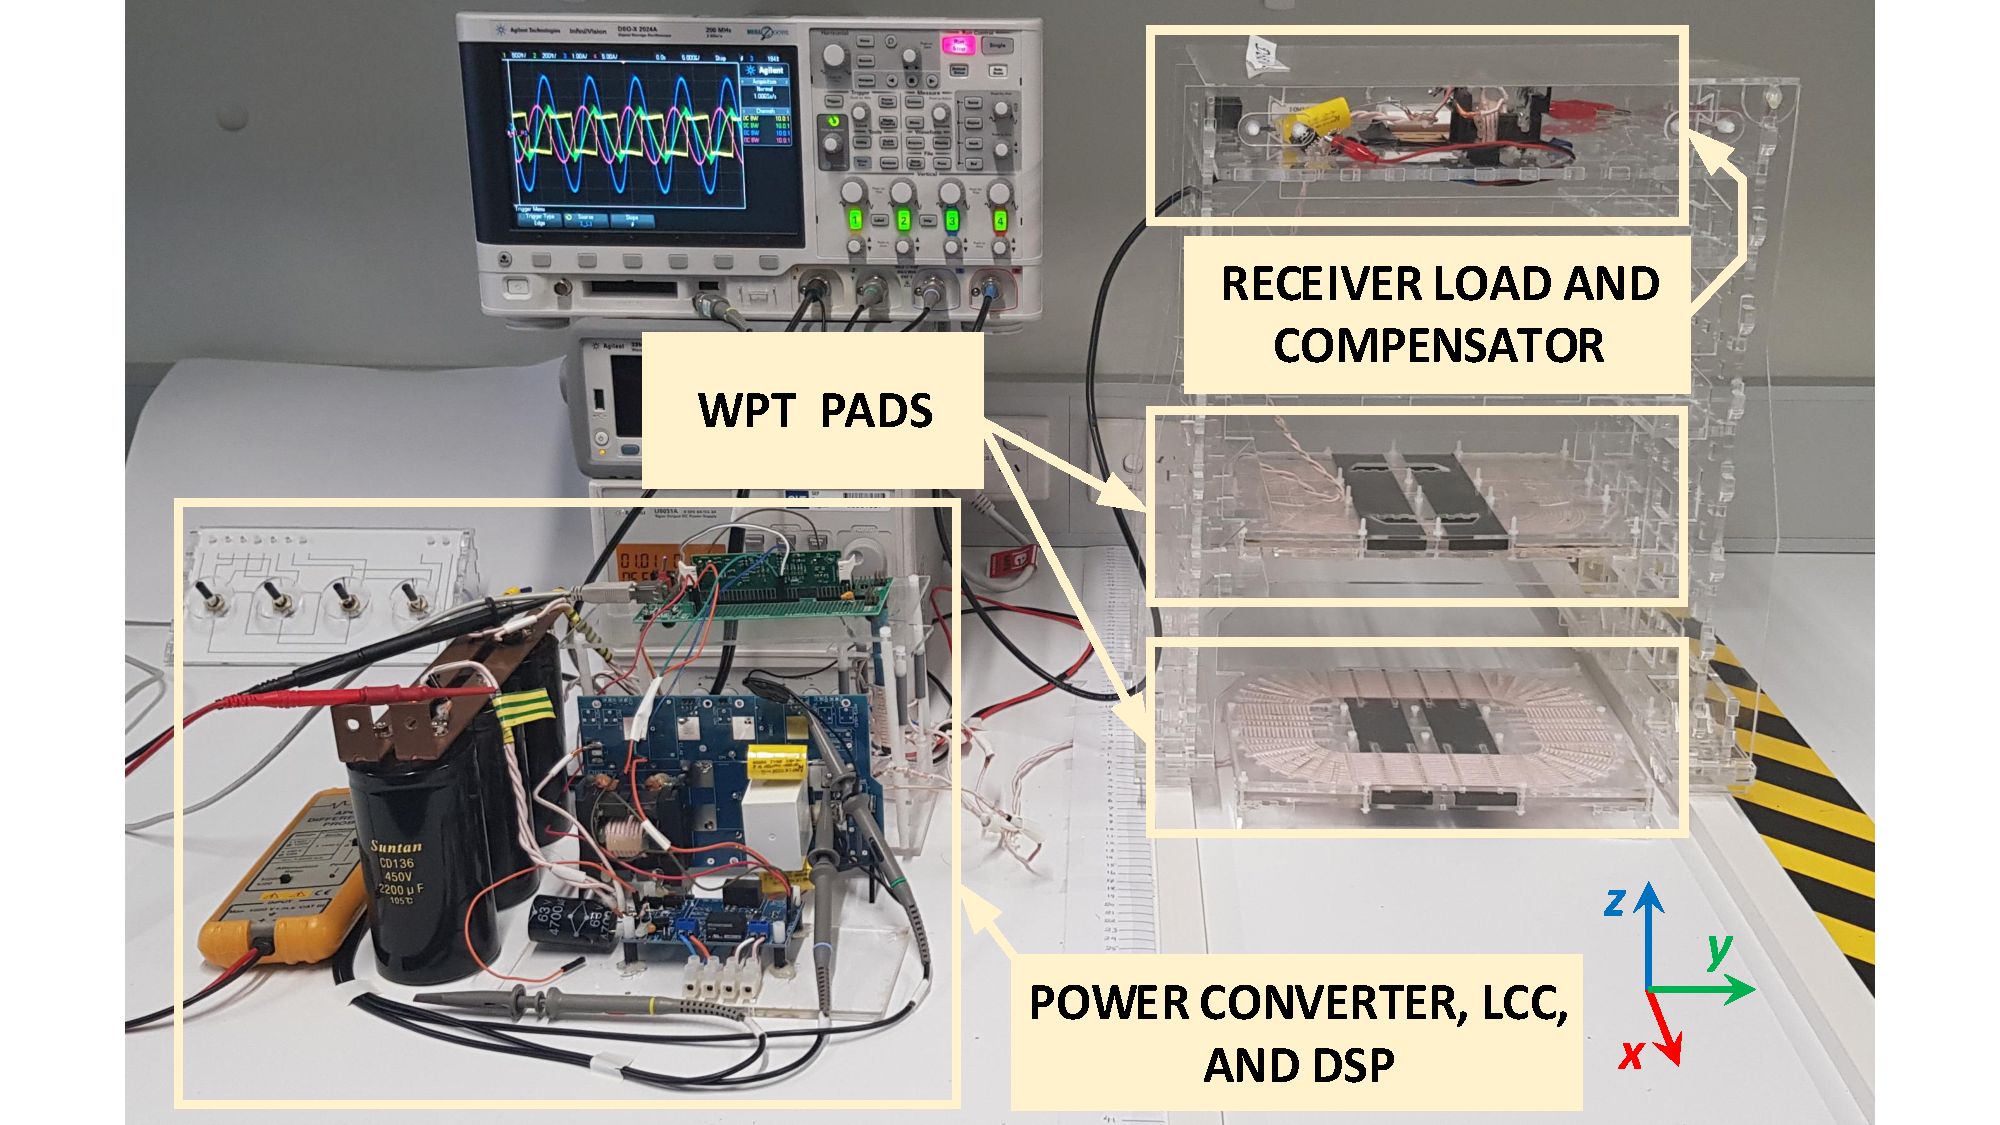
\includegraphics[clip, trim=.7cm 0cm 0cm 0cm, width=1\columnwidth]{Figs/Fig9_a.pdf}
    }\\ \vspace{-3mm}
    \subfloat[]{
        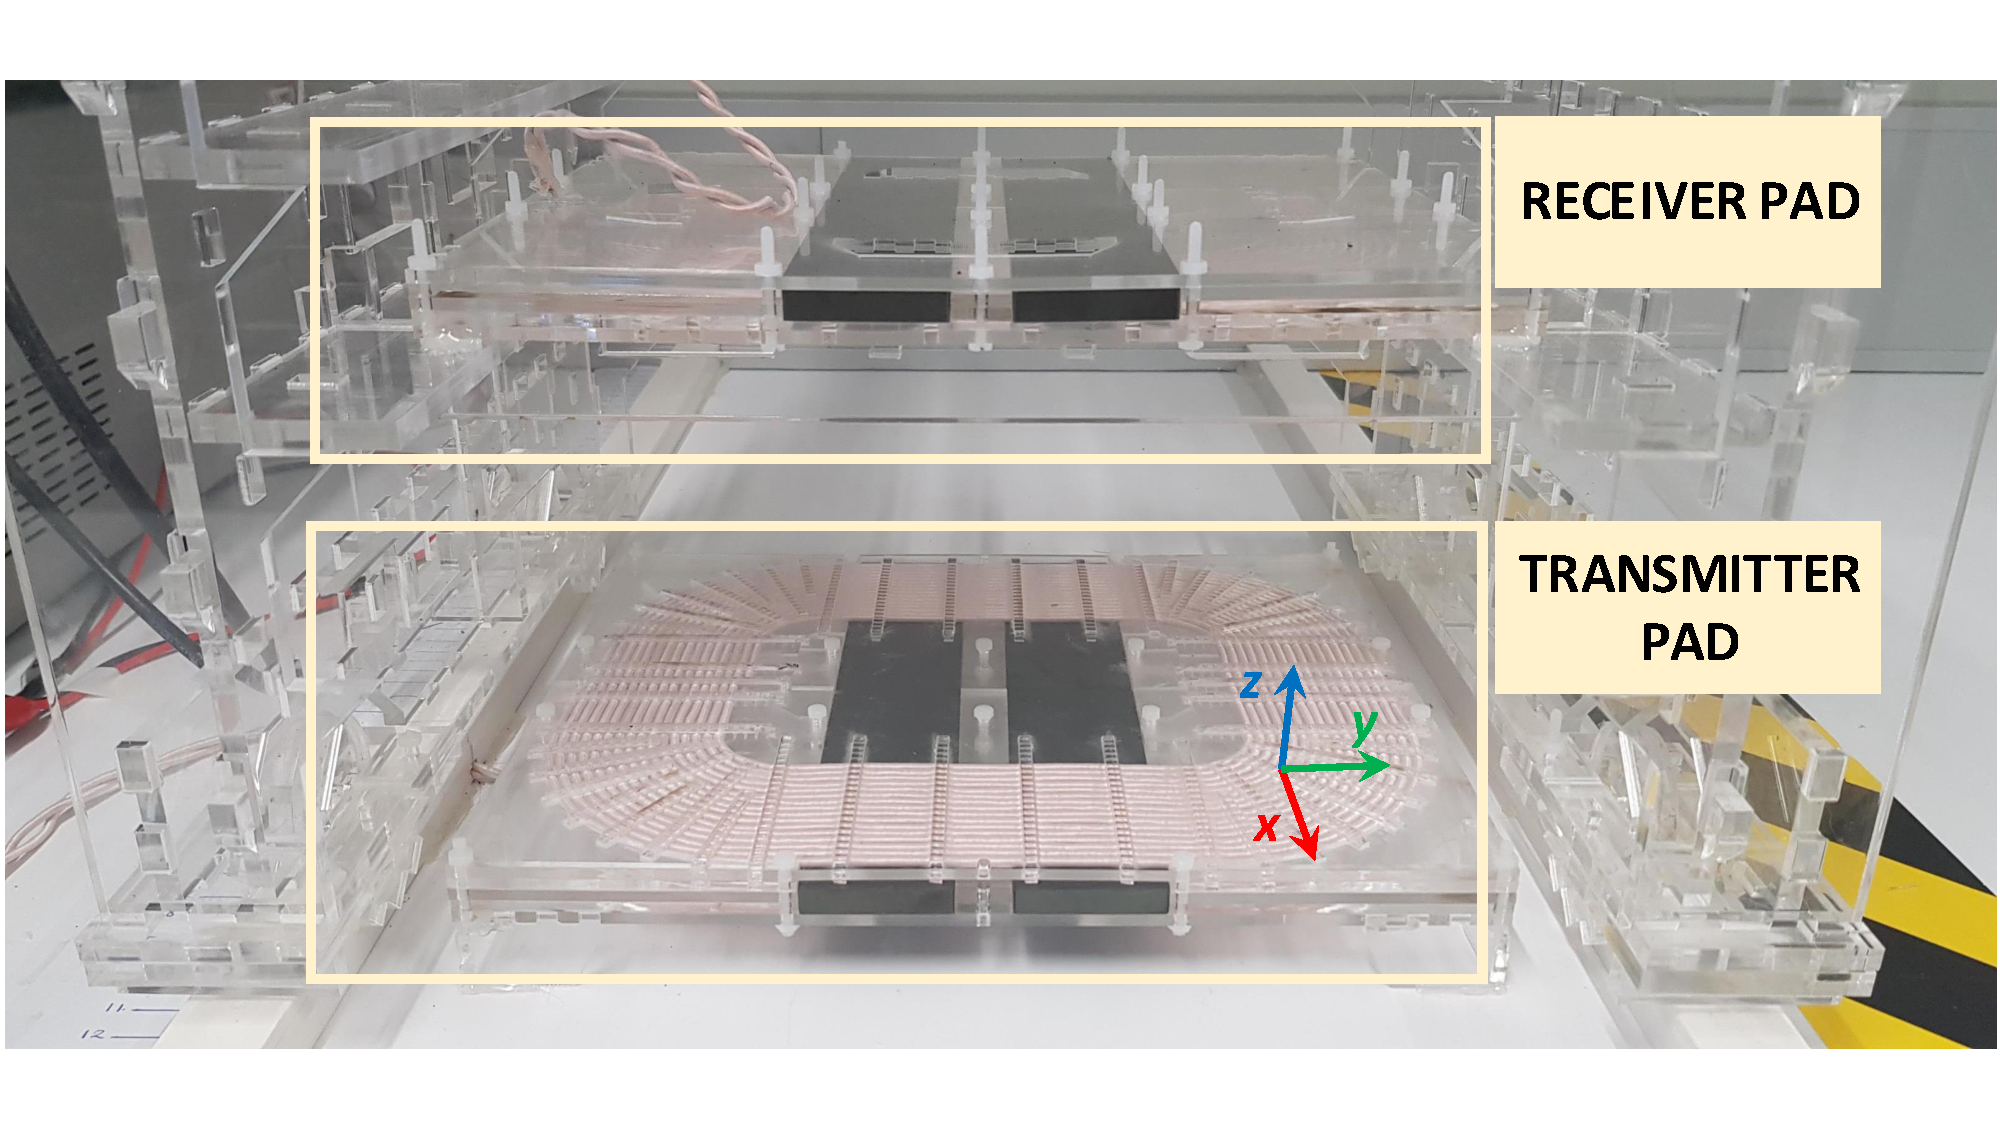
\includegraphics[clip, trim=0cm 1cm 0cm 1cm, width=.9\columnwidth]{Figs/Fig9_b.pdf}
    }\\ \vspace{-3mm}
    \subfloat[]{
        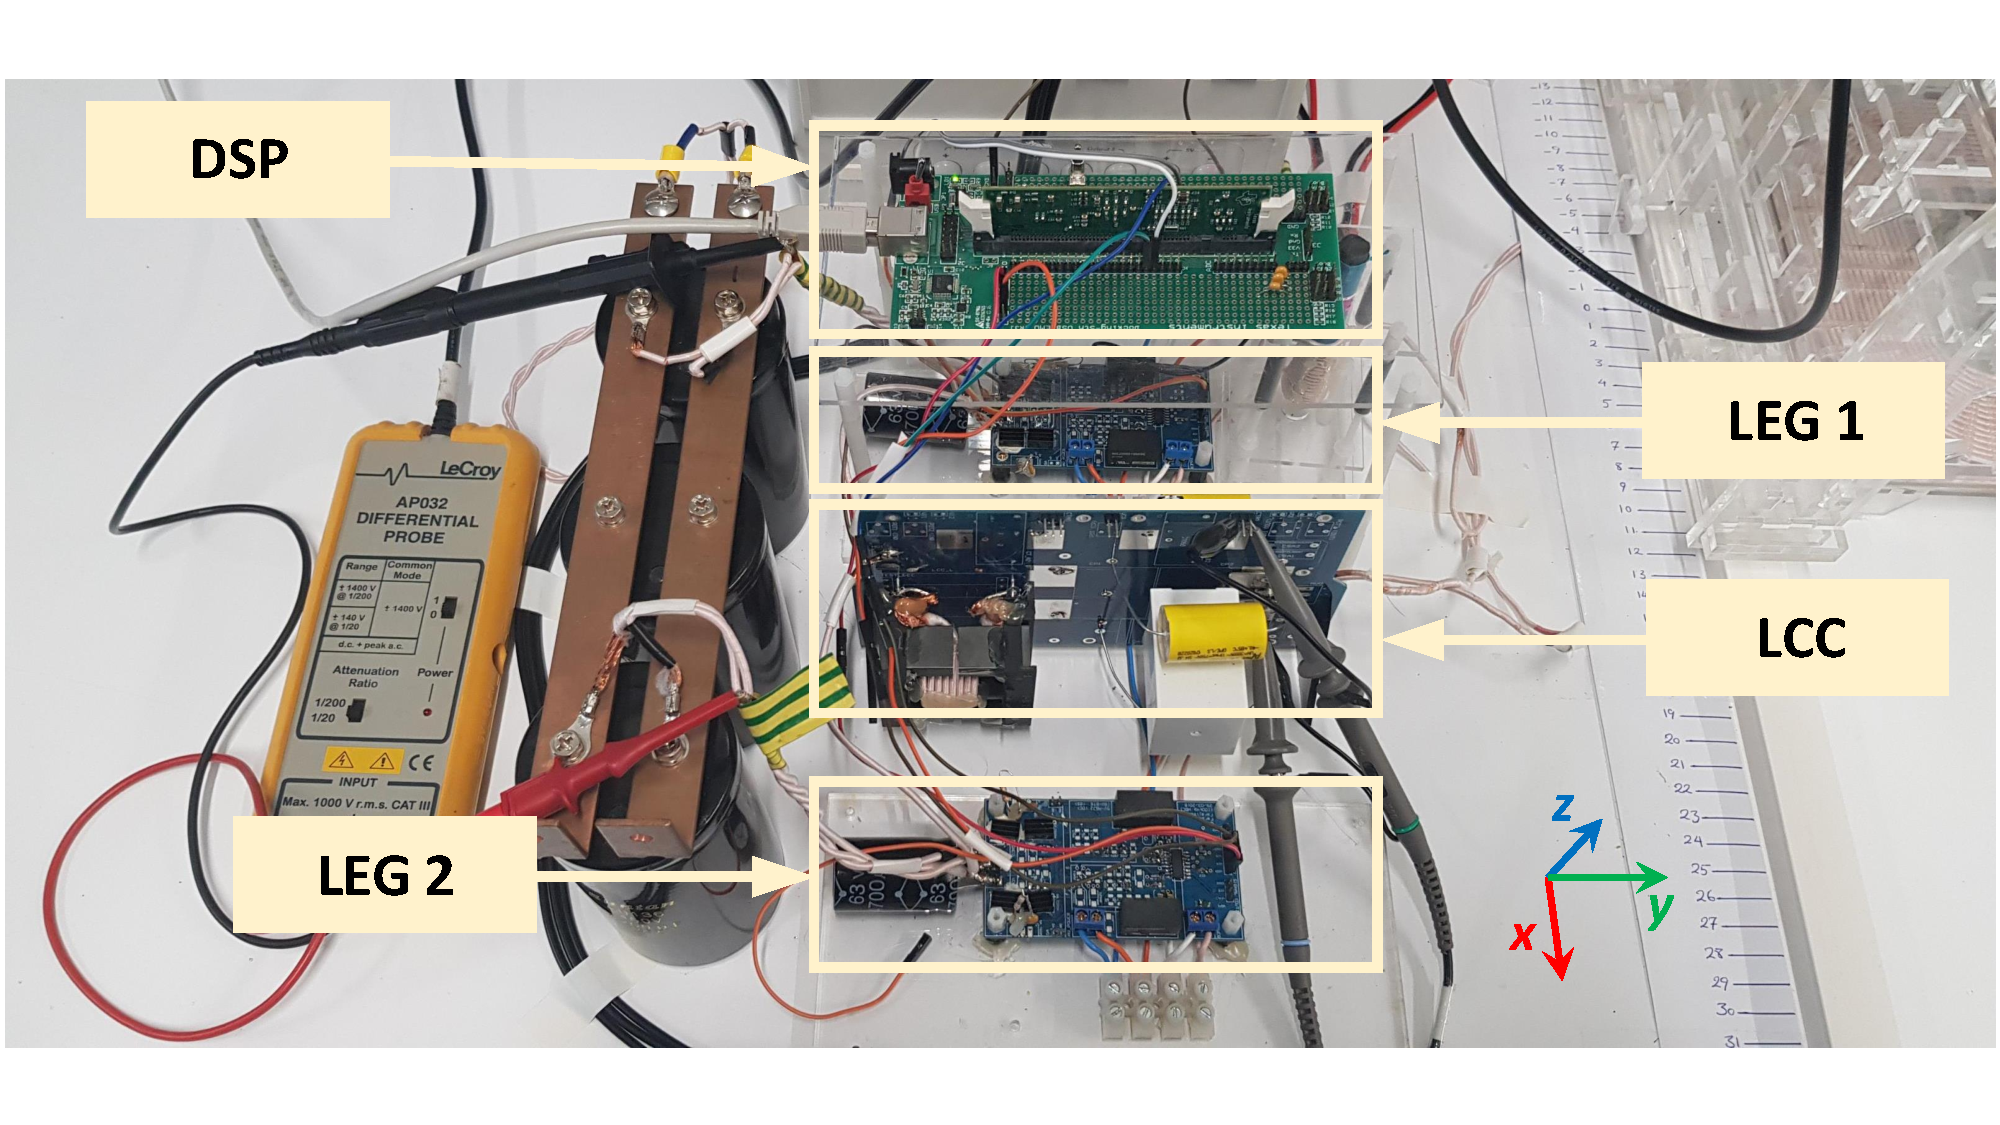
\includegraphics[clip, trim=0cm 1cm 0cm 1cm, width=.9\columnwidth]{Figs/Fig9_c.pdf}
        \vspace{-3mm}
    }
\end{center}
\vspace{-3mm}
	\caption{The experimental setup; (a) whole the setup, (b) WPT pads, and (c) transmitter driving system.}
		\label{Fig.Fig9}
		\vspace{-3mm}
\end{figure}
%%

%%FIG11
\begin{figure}[t!]
\begin{center}
	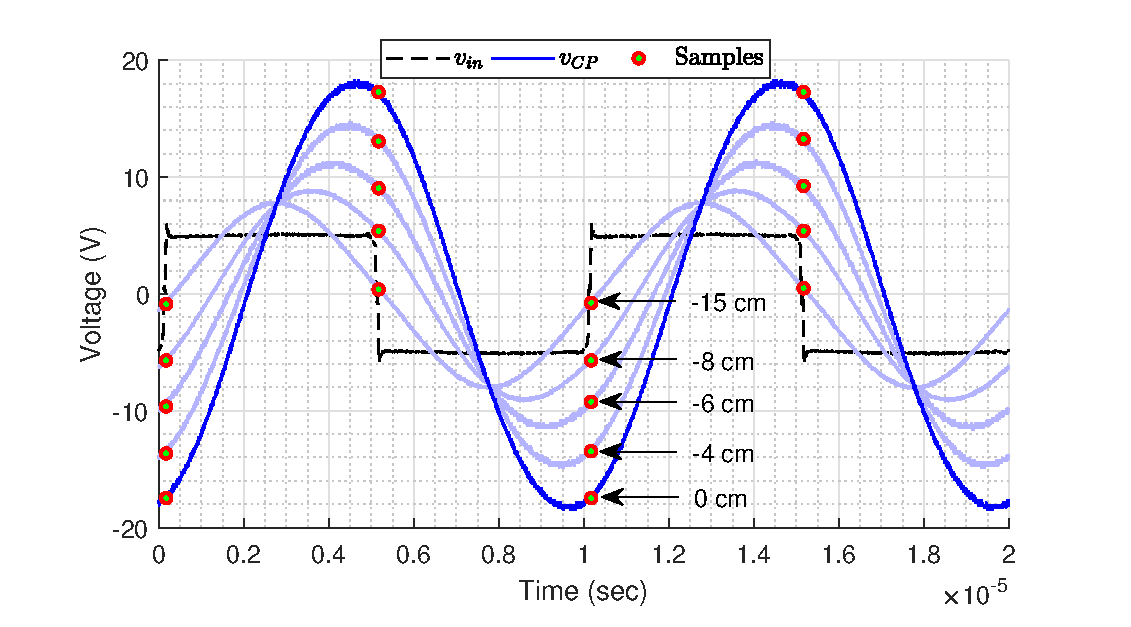
\includegraphics[clip, trim=1cm 0.0cm 1cm 0cm, width=1\columnwidth]{Figs/Fig10.eps}
\end{center}
\vspace{-0.1cm}
	\caption{$v_\textrm{\rm in}$, $v_\textrm{CP}$, and $v_\textrm{CP}$ PWM-synchronized samples at five different receiver positions for $R_{\mathrm{L}}=1 \Omega$.}
		\label{Fig.Fig10}
		%\vspace{-3mm}
		\vspace{-3mm}
\end{figure}
%%
\newline
Having the measured transmitter-receiver mutual inductance ($L_{\mathrm{TR}}$), load at the receiver ($R_{\mathrm{L}}$), LCC series inductance ($L_{\mathrm{S}}$) and with the use of \eqref{EQ.EQ.4}, the actual demand factor ($\xi^*$) is calculated, and the results are shown in Fig.~\ref{Fig.Fig11}. In this figure, the experimental result of the estimated demand factor ($\xi_{\mathrm{est}}$) obtained from PWM-synchronized sampling is also shown for the comparison.

%%FIG11
\begin{figure}[t!]
\begin{center}
	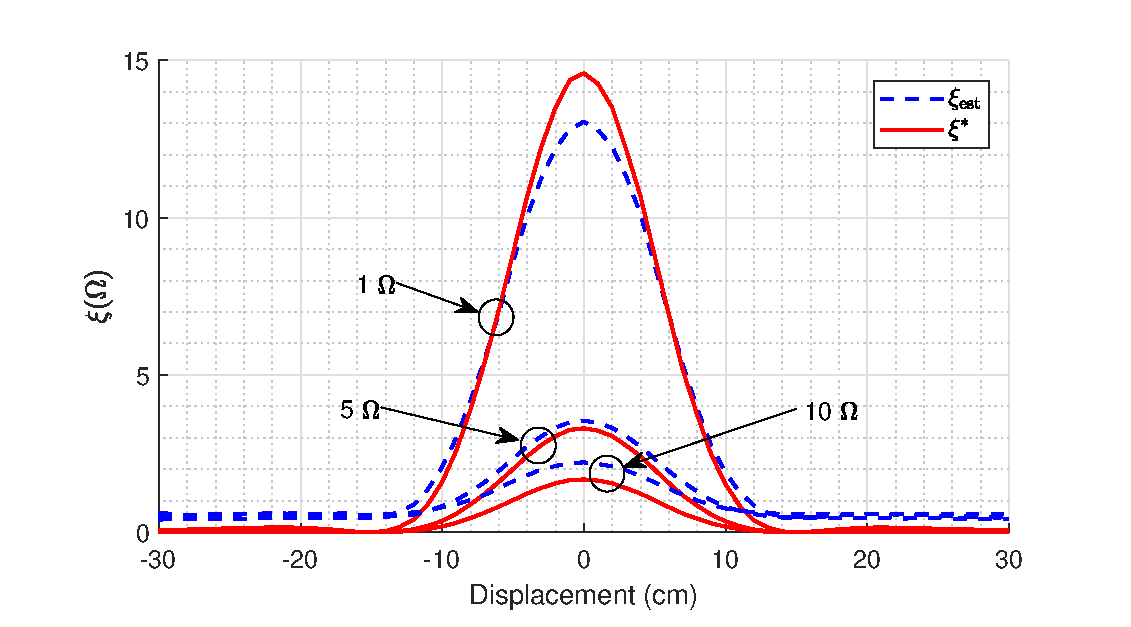
\includegraphics[clip, trim=1cm 0.0cm 1cm 0.0cm, width=1\columnwidth]{Figs/Fig11.eps}
\end{center}
\vspace{-0.1cm}
	\caption{Experimental results for the estimated ($\xi_{\mathrm{est}}$) and actual ($\xi^*$) demand factors for different positions of the receiver.}
		\label{Fig.Fig11}
		%\vspace{-5mm}
		\vspace{-3mm}
\end{figure}
%%

In a similar way, the output power ($P_{\rm out}$) and input power ($P_{\rm in}$) have been experimentally measured at different positions, and, subsequently, the efficiency profile has been obtained as shown in Figs.~\ref{Fig.Fig12} and \ref{Fig.Fig13}.

%%Fig12
\begin{figure}[t!]
\begin{center}
	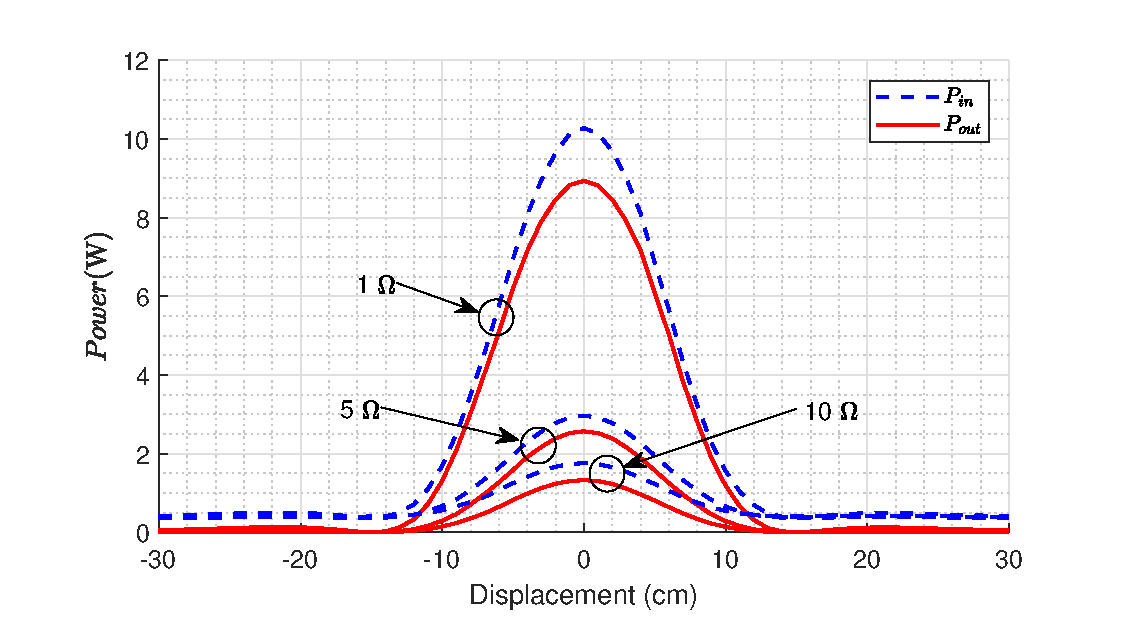
\includegraphics[clip, trim=1cm 0.0cm 1cm 0.0cm, width=1\columnwidth]{Figs/Fig12.eps}
\end{center}
\vspace{-0.1cm}
	\caption{Experimental results for the output and input powers for different positions of the receiver.}
		\label{Fig.Fig12}
		\vspace{-3mm}
\end{figure}
%%

%%Fig13
\begin{figure}[t!]
\begin{center}
	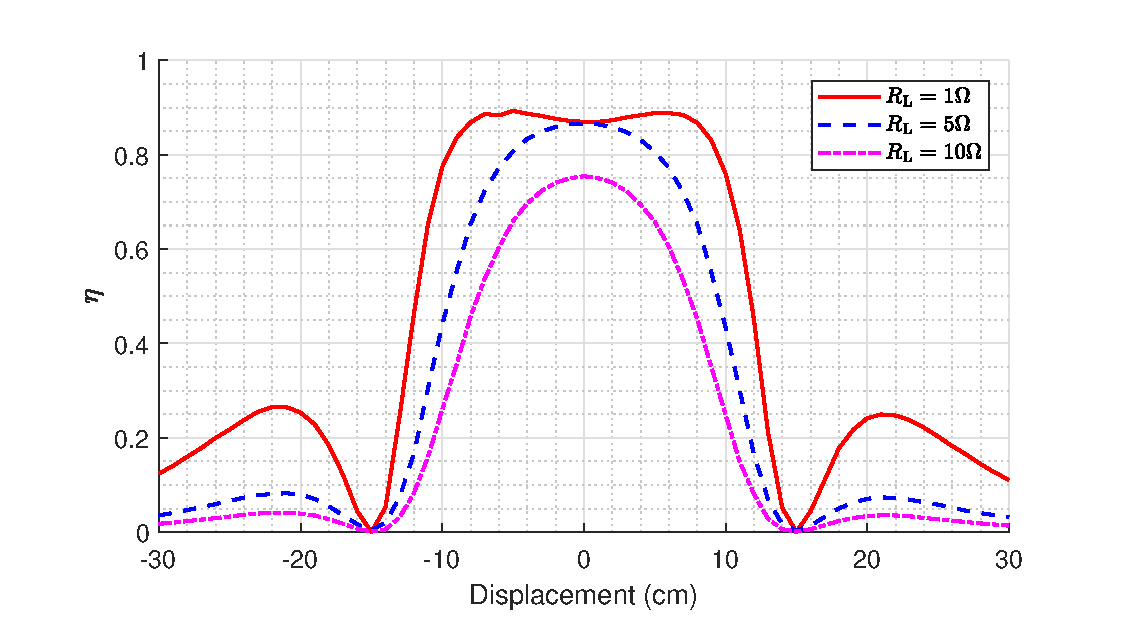
\includegraphics[clip, trim=1cm 0.0cm 1cm 0.0cm, width=1\columnwidth]{Figs/Fig13.eps}
\end{center}
\vspace{-0.1cm}
	\caption{Experimental results for the efficiency ($\eta$) for different positions of the receiver.}
		\label{Fig.Fig13}
		\vspace{-3mm}
\end{figure}
%%

To combine the effect of transmitter-receiver mutual inductance ($L_{\mathrm{TR}}$) and load variations ($R_{\mathrm{L}}$) for different displacements ($x$) and loads ($R_{\mathrm{L}}$), the variation of the experimentally estimated error ($e_{\mathrm{est}}$) versus efficiency ($\eta$) is depicted and compared with the numerical results in Fig.~\ref{Fig.Fig14}.

%%Fig14
\begin{figure}[t!]
\begin{center}
	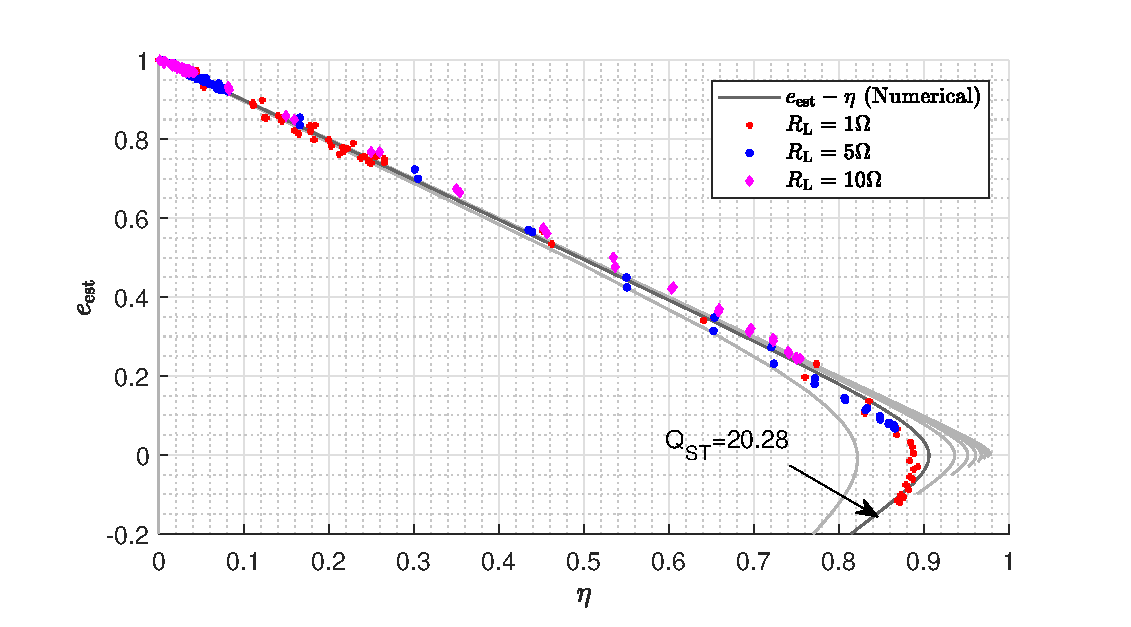
\includegraphics[clip, trim=1cm 0.0cm 1cm 0.0cm, width=1\columnwidth]{Figs/Fig14.eps}
\end{center}
\vspace{-0.1cm}
	\caption{Experimental and numerical results for the variation of the estimated error ($e_{\mathrm{est}}$) versus efficiency ($\eta$).}
		\label{Fig.Fig14}
		\vspace{-3mm}
\end{figure}
%%
From Fig.~\ref{Fig.Fig11}, it can be seen that the estimated demand factor ($\xi_{\mathrm{est}}$) follows the actual demand factor ($\xi^*$) in a reasonable way. Moreover, Fig.~\ref{Fig.Fig14} shows that the experimental results are completely in accordance with the numerical results, and it follows the $e_{\mathrm{est}}-\eta$ pattern for $Q_{\mathrm{ST}}=20.28$.
Fig.~\ref{Fig.Fig14} also explains that the higher the efficiency, the lower the estimated error, which means this method can accurately observe the flow of power when transmitter and receiver are effectively coupled. On the other hand, the lack of accuracy happens when the efficiency is low, which occurs when the transmitter-receiver coupling is low. This, however, cannot be inferred as a major drawback, as the operation of WPT systems at low efficiencies is not desirable, and transmitter pads are preferred to be turned OFF at those conditions where the estimated demand factor is low (high estimated errors). Furthermore, by putting the transmitter in the idle mode of operation (transmission of a low amount of power only to detect the presence of the receiver), the presence of the receiver can still be detected at the low accuracy zone of this approach. This can be done owing to the meaningful variation of the estimated demand factor when the receiver approaches the transmitter, even when the coupling is low (low efficiencies). Therefore, although for low couplings the estimated error is high, this method can still be used to detect the effective range of the receiver displacement to activate or deactivate the transmitters.

\section{Conclusion}
In this paper, a new approach to observe the transferred power in WPT systems is presented. Taking the PWM-synchronized samples from the front-end variables of the LCC compensator makes this technique a simple and feasible way to be used in different applications. The mathematical equations linking the transferred power (which is received by the receiver) to the front-end variables are derived, and it is shown that the transferred power can be observed by taking the PWM-synchronized samples from the LCC parallel capacitor. Then, by considering the effect of dominant equivalent resistances in the system, the accuracy of this system is characterized. Finally, the close correlation between the numerical and experimental results confirms the proposed technique.





% if have a single appendix:
%\appendix[Proof of the Zonklar Equations]
% or
%\appendix  % for no appendix heading
% do not use \section anymore after \appendix, only \section*
% is possibly needed

% use appendices with more than one appendix
% then use \section to start each appendix
% you must declare a \section before using any
% \subsection or using \label (\appendices by itself
% starts a section numbered zero.)
%

%\newpage
\appendix
\begin{table}[!h]
\vspace{-3mm}
\renewcommand{\arraystretch}{1.3}
\caption{Simulation and Experimental Specifications.}
\centering
\label{TBL1}
	    \vspace{-2mm}
	    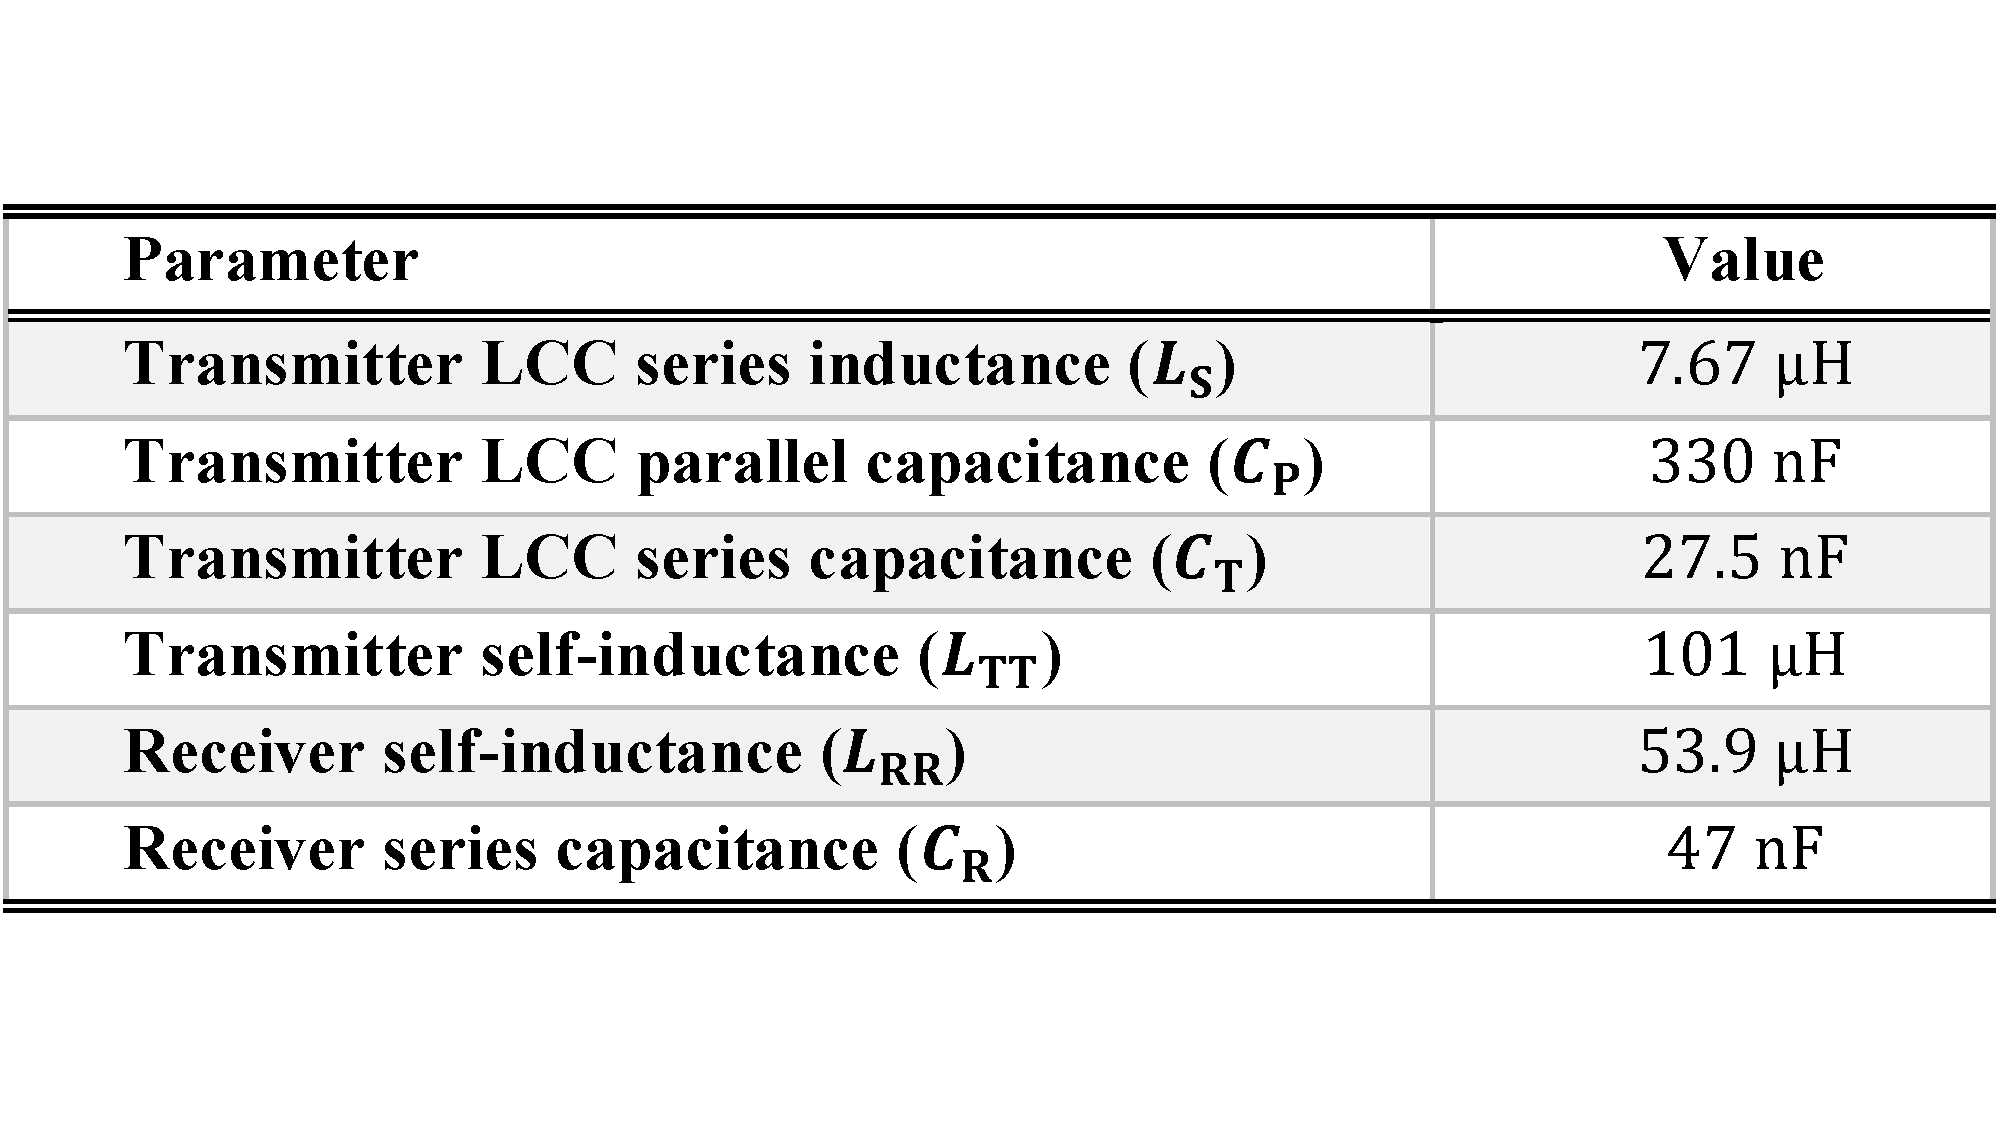
\includegraphics[clip,trim= 0cm 3.5cm 0cm 3.5cm,width=0.95\columnwidth]{Figs/TBL1.pdf}
% \begin{tabular}{lc}
% \toprule\toprule
% Parameter                                               &       Value \\ \midrule
% Transmitter Self-Inductance ($L_\mathrm{TT}$)           &       ?? $\mathrm{\mu H}$ \\
% LSS Series Inductance ($L_\mathrm{S}$)                  &       7.5 $\mathrm{\mu H}$ \\
% Transmitter LCC Parallel Capacitance ($C_\mathrm{P}$)   &       330 $\mathrm{nF}$ \\
% Transmitter LCC Series Capacitance ($C_\mathrm{T}$)     &       ?? $\mathrm{nF}$ \\
% Receiver Self-Inductance ($L_\mathrm{RR}$)              &       ?? $\mathrm{\mu H}$ \\
% Receiver Series Capacitance ($C_\mathrm{S,T}$)          &       ?? $\mathrm{\mu H}$ \\
% Receiver Load ($R_\mathrm{L}$)                          &       ?? $\mathrm{\mu H}$ \\
% \bottomrule\bottomrule
% \end{tabular}
\vspace{-5mm}
\end{table}

\ifCLASSOPTIONcaptionsoff
  \newpage
\fi



% trigger a \newpage just before the given reference
% number - used to balance the columns on the last page
% adjust value as needed - may need to be readjusted if
% the document is modified later
%\IEEEtriggeratref{8}
% The "triggered" command can be changed if desired:
%\IEEEtriggercmd{\enlargethispage{-5in}}

% references section

% can use a bibliography generated by BibTeX as a .bbl file
% BibTeX documentation can be easily obtained at:
% http://mirror.ctan.org/biblio/bibtex/contrib/doc/
% The IEEEtran BibTeX style support page is at:
% http://www.michaelshell.org/tex/ieeetran/bibtex/
%\bibliographystyle{IEEEtran}
% argument is your BibTeX string definitions and bibliography database(s)
%\bibliography{IEEEabrv,../bib/paper}
%
% <OR> manually copy in the resultant .bbl file
% set second argument of \begin to the number of references
% (used to reserve space for the reference number labels box)

%\bibitem{IEEEhowto:kopka}
%H.~Kopka and P.~W. Daly, \emph{A Guide to \LaTeX}, 3rd~ed.\hskip 1em plus
%  0.5em minus 0.4em\relax Harlow, England: Addison-Wesley, 1999.

\bibliographystyle{IEEEtran}% bib style
%\bstctlcite{IEEEexample:BSTcontrol}
\bibliography{Bibliography}% your bib database
% that's all folks
\end{document}


% biography section
% 
% If you have an EPS/PDF photo (graphicx package needed) extra braces are
% needed around the contents of the optional argument to biography to prevent
% the LaTeX parser from getting confused when it sees the complicated
% \includegraphics command within an optional argument. (You could create
% your own custom macro containing the \includegraphics command to make things
% simpler here.)
\begin{IEEEbiography}[{
\includegraphics[width=1in,height=1.25in,clip,keepaspectratio]{Figs/Donkey.jpg}}]{Test}
% or if you just want to reserve a space for a photo:

%\begin{IEEEbiography}{Michael Shell}
Biography text here.
\end{IEEEbiography}

% if you will not have a photo at all:
\begin{IEEEbiographynophoto}{John Doe}
Biography text here.
\end{IEEEbiographynophoto}

% insert where needed to balance the two columns on the last page with
% biographies
%\newpage

\begin{IEEEbiographynophoto}{Jane Doe}
Biography text here.
\end{IEEEbiographynophoto}

% You can push biographies down or up by placing
% a \vfill before or after them. The appropriate
% use of \vfill depends on what kind of text is
% on the last page and whether or not the columns
% are being equalized.

%\vfill

% Can be used to pull up biographies so that the bottom of the last one
% is flush with the other column.
%\enlargethispage{-5in}



% that's all folks
\end{document}


